\documentclass{article}

\usepackage[left=100pt,right=100pt]{geometry}
\usepackage[round]{natbib}
\usepackage[french]{babel}
\usepackage[utf8]{inputenc}
\usepackage[T1]{fontenc}
\usepackage{float}
\usepackage{graphicx}
\usepackage{multicol}
\usepackage{caption}
\usepackage{subcaption}
\usepackage{mathtools}
\usepackage{afterpage}
\usepackage[normalem]{ulem}
\usepackage{listings}
\usepackage{xcolor}
\usepackage{hyperref}

% Pour l'ajout de Watermark
% \usepackage[printwatermark]{xwatermark}
% \usepackage{lipsum}
% \newwatermark[allpages,color=gray!20,angle=45,scale=3,xpos=0,ypos=0]{NAME}


% Formattage des hyperliens
\hypersetup{
    colorlinks=true,
    linkcolor=black,
    filecolor=black,
    urlcolor=black,
    citecolor=black
}
\urlstyle{same}

% Change la mise en page des segments de codes
\definecolor{codegreen}{rgb}{0,0.6,0}
\definecolor{codegray}{rgb}{0.2,0.2,0.2}
\definecolor{codepurple}{rgb}{0.58,0,0.82}
\definecolor{backcolour}{rgb}{0.95,0.95,0.95}
\lstdefinestyle{mystyle}{
    backgroundcolor=\color{backcolour},
    commentstyle=\color{codegreen},
    keywordstyle=\color{magenta},
    numberstyle=\tiny\color{codegray},
    stringstyle=\color{codepurple},
    basicstyle=\ttfamily\footnotesize,
    breakatwhitespace=false,
    breaklines=true,
    captionpos=b,
    keepspaces=true,
    numbers=left,
    numbersep=5pt,
    showspaces=false,
    showstringspaces=false,
    showtabs=false,
    tabsize=4
}
\lstset{style=mystyle}

\renewcommand{\contentsname}{Table des matières}
\renewcommand{\listfigurename}{Table des figures}
\renewcommand{\refname}{Bibliographie}
\renewcommand{\lstlistingname}{Segment de codes}
\renewcommand{\lstlistlistingname}{Table des segments de code}

\bibliographystyle{plainnat}

\setlength\parindent{0pt} % Enleve les indentations dans le document

\title{Laboratoire 1\\
  \large Perceptron multicouche (MLP)\\
  \normalsize Durée : 1 séance}
\author{Par Chakib Tadj et Christophe Lamarche}
\date{mise à jour: \today}


\begin{document}
\maketitle

\section{Description}
Ce laboratoire a comme but de s'initier avec le langage informatique \textbf{Python}, l'environnement de programmation \textbf{Colaboratory} et les librairies utilisées dans la conception de réseaux neuronaux.

\medbreak
Les réseaux de neurones conçus durant ce laboratoire devront extraire les paramètres les plus pertinents d'un signal de parole et réaliser la reconnaissance de la parole. Ce laboratoire consiste en la conception d'un réseau de neurones à rétropropagation du gradient de l'erreur (\textit{Descente du gradient stochastique} [SGD]).

\subsection{Exposé du problème}
La difficulté du processus de traitement du signal de la parole réside dans la nature même de ce signal qui est pseudo-aléatoire. De ce fait, l'extraction des paramètres temporels de l'information contenus dans celui-ci devient problématique. Une façon de solutionner le problème est d'en extraire les paramètres les plus pertinents dans le domaine des fréquences. La FFT (Fast Fourier Transform / Transformée de Fourier Rapide) est un outil qui est largement utilisé dans ce domaine pour représenter le signal temporel en fréquence. En général, on filtre le signal sur une série de bancs de filtres selon une échelle logarithmique. Ceci est justifié par le fait que le système auditif humain est logarithmique quant à sa capacité de percevoir les plages de fréquences. Une fois les paramètres les plus pertinents du signal extrait (figure \ref{fig:traitement_signal}), ils sont utilisés pour entraîner le réseau de neurones. La tâche de celui-ci consiste à projeter les données dans un espace de dimension réduite permettant une meilleure discrimination entre les différentes formes du signal de parole.

\begin{figure}[H]
  \centering
  \fbox{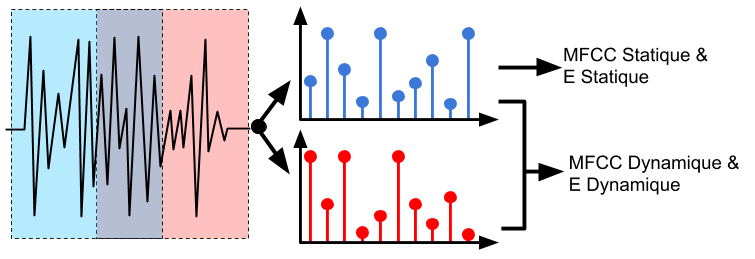
\includegraphics[width=0.75\linewidth]{figures/traitement_signal}}
  \caption{Traitement du signal audio}
  \label{fig:traitement_signal}
\end{figure}

\bigbreak
Les données à l'intérieur des bases de données sont divisées en 60 fenêtres. Chaque fenêtre possède 12 MFCCs (\textit{coefficients Cepstraux à Fréquences Mel}) statiques, une valeur de l'énergie statique, 12 MFCCs dynamiques et une valeur de l'énergie dynamique. Donc, chaque signal sonore possède 1560 coefficients et le chiffre lié au signal.

$$1560 = 60[\text{fenêtres}]\cdot(12[\text{MFFC statique}]+1[\text{E statique}]+12[\text{MFCC dynamique}]+1[\text{E dynamique}])$$

\bigbreak
Pour se faire, l'étudiant devra concevoir et analyser les performances de quatre réseaux de neurones afin de classifier les segments audios.
\begin{itemize}
  \item Perceptron simple
  \item MLP de 2 couches
  \item MLP de 2 couches avec couche d'abandon (\textit{Dropout})
  \item MLP de 3 couches
\end{itemize}

\section{Théorie}
\subsection{Python}
Python est un langage de programmation orienté objet qui a eu un gain de popularité lors de son appropriation par le secteur de l'analyse de données (\textit{Data Science}). Il est souvent décrit comme un langage de programmation facile à apprendre. L'utilisation de Python s'étend de la conception d'applications web à la création de réseaux neuronaux en passant par la création de jeux video. Python à l'aide de la librairie \textit{Numpy} peut être utilisé afin de faire des calculs numériques similaires avec ce qui peut être fait avec \textit{MATLAB}.
\subsection{\href{https://colab.research.google.com/}{Colaboratory}}

Colaboratory est un environnement de programmation de type \textit{Notebook} basé sur le \textit{Project Jupyter}. Cet environnement est offert en ligne gratuitement pour quiconque (utilisation personnelle et utilisation professionnelle). Il intègre plusieurs des librairies d'apprentissage machine et met à la disposition de l'usager des GPUs (\textit{Graphical Processing Unit}) et des TPUs (\textit{Tensor Processing Unit}) pour accélérer l'entraînement des modèles.

\subsection{Tensorflow}
\textbf{Tensorflow} est une librairie d'apprentissage machine \textit{Open Source} basée sur la librairie \textbf{Keras}. Tensorflow offre la possibilité d'embarquer les modèles pour le web (avec tensorflow.js), les applications mobiles (avec Tensorflow Lite) et en production avec (Tensorflow Extended).

\subsection{Autres librairies utilisées}

\begin{itemize}
  \item \href{https://www.tensorflow.org/api_docs/python/tf/keras/layers}{Tensorflow.keras.layer}:
    \begin{itemize}
      \item Module de Tensorflow offrant les différentes couches qui seront intégrées dans le réseau
    \end{itemize}
  \item \href{https://numpy.org/doc/stable/user/numpy-for-matlab-users.html}{Numpy}:
    \begin{itemize}
      \item Librairie mathématique (La plus utilisée de Python)
      \item Elle est utilisée pour faciliter la manipulation de tableau
    \end{itemize}
  \item \href{https://pandas.pydata.org/docs/getting_started/index.html#getting-started}{Pandas}:
    \begin{itemize}
      \item Librairie pour manipuler des bases de données (Dataframes)
      \item Elle est utilisée pour importer les bases de données ".csv"
    \end{itemize}
  \item \href{https://matplotlib.org/gallery/index.html#}{Matplotlib.pyplot}:
    \begin{itemize}
      \item Librairie d'affichage graphique
      \item Elle est utilisée pour la production de graphique et de tableau
    \end{itemize}
  \item \href{https://scikit-learn.org/stable/auto_examples/index.html#}{Sklearn}:
    \begin{itemize}
      \item Librairie d'apprentissage machine
      \item Elle est utilisée pour la segmentation de la base de données d'entraînement avec KFold
    \end{itemize}
  \item \href{https://docs.scipy.org/doc/scipy/reference/stats.html}{Scipy.stats}:
    \begin{itemize}
      \item Regroupement de librairies de mathématique, de science et d'ingénierie
      \item Elle est utilisée pour calculer le mode des résultats des modèles pour déterminer la valeur à l'intérieur de la base de données mystère.
    \end{itemize}
\end{itemize}

\section{Étapes} % Enumerer les étapes pour concevoir le laboratoire
\subsection{Ouvrir un Notebook}
Afin d'ouvrir un Notebook, il est préférable d'utiliser le navigateur Chrome. Toutefois, l'environnement est fonctionnel sur d'autres navigateurs.
\medbreak
Colaboratory est accessible à l'URL : `\href{https://colab.research.google.com/}{https://colab.research.google.com/}. Afin de créer un nouvel environnement, il est nécessaire de se connecter avec un compte Google/Gmail.
\medbreak
Sur le site, vous êtes reçu par la figure \ref{fig:start}. Choisissez l'option `NEW NOTEBOOK'. Cette action démarre un notebook contenant une cellule de code tel qu'à la figure \ref{fig:open}. Dans le cas où vous êtes reçu par un notebook nommé ``\textit{Welcome to Colaboratory}'', assurez-vous que vous êtes bien connecté sur votre compte Google et sous l'onglet Fichier (\textit{File}), sélectionnez l'objet `Nouveau notebook' (\textit{New Notebook}).

\begin{figure}[H]
  \centering
  \fbox{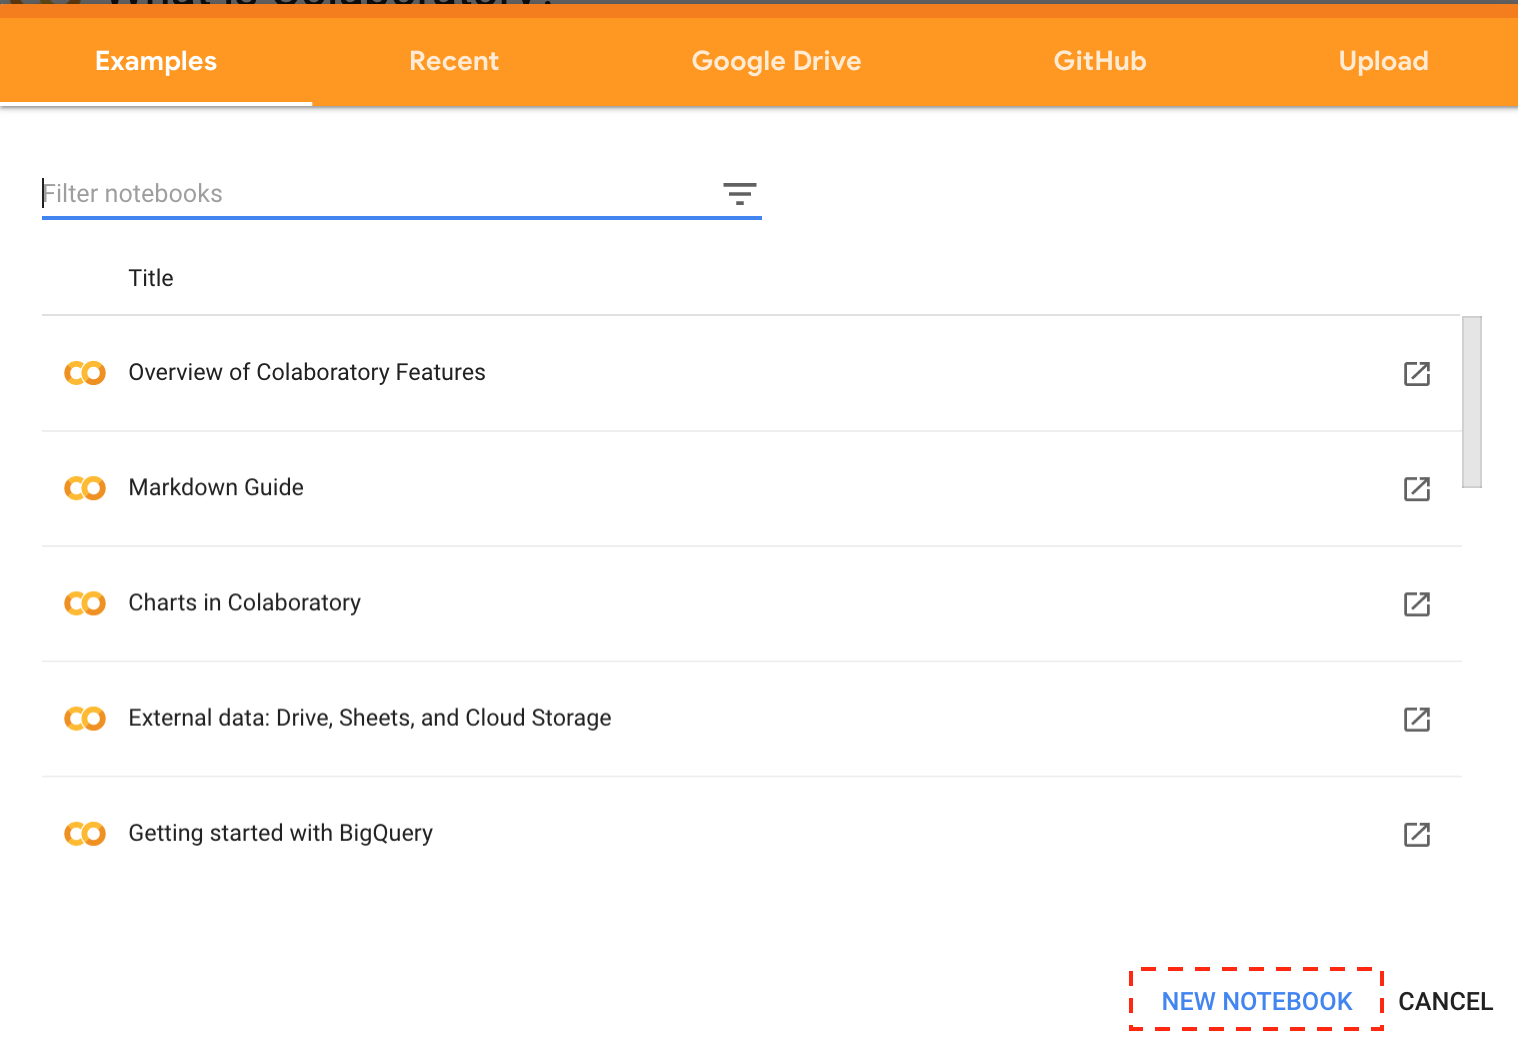
\includegraphics[width=0.75\linewidth]{figures/starting_menu}}
  \caption{Menu de départ}
  \label{fig:start}
\end{figure}


\begin{figure}[H]
  \centering
  \fbox{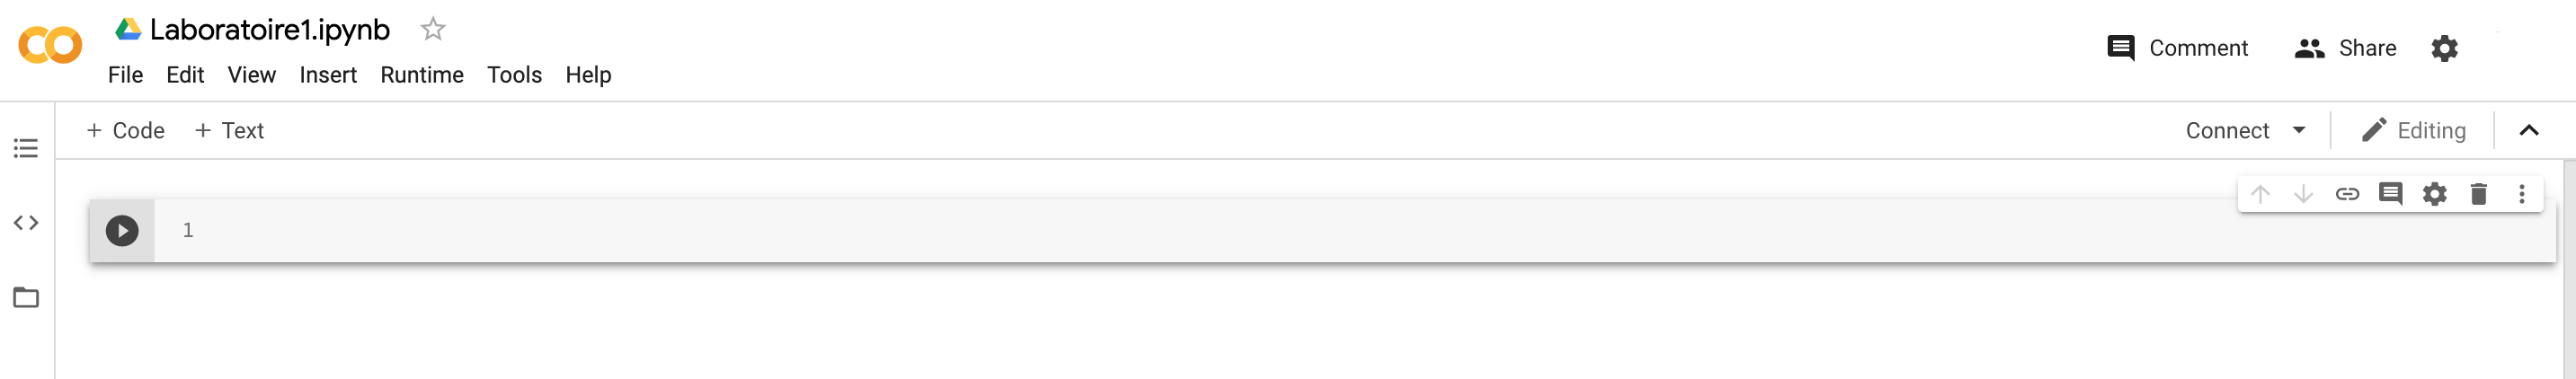
\includegraphics[width=0.75\linewidth]{figures/openning_screen}}
  \caption{Notebook de départ}
  \label{fig:open}
\end{figure}

\subsection{Personnaliser le Notebook}
Avant de commencer, il peut être intéressant de personnaliser le notebook afin d'améliorer l'expérience. Les étapes suivantes ne sont pas obligatoires, mais elles sont conseillées.
\medbreak

Sous l'onglet `Outils' (\textit{Tools}), cliquer sur l'option `Paramètres' (\textit{Settings}) (figure \ref{fig:setting}). Il est possible d'accéder le menu `Paramètres' avec l'icône d'engrenage en haut à droite du notebook ou en haut à droite des cellules du notebook.

\begin{figure}[H]
  \centering
  \fbox{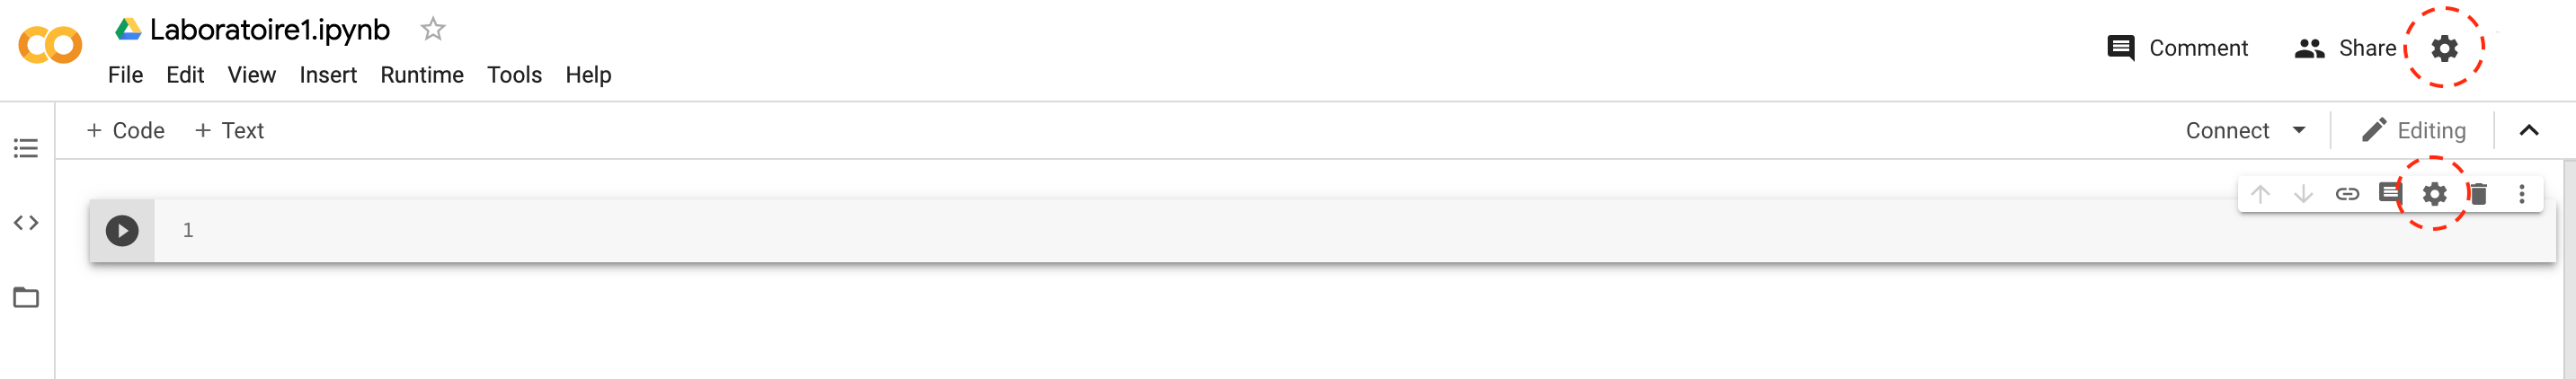
\includegraphics[width=0.75\linewidth]{figures/setting_position}}
  \caption{Position des icônes des paramètres}
  \label{fig:setting_position}
\end{figure}

\begin{figure}[H]
  \centering
  \fbox{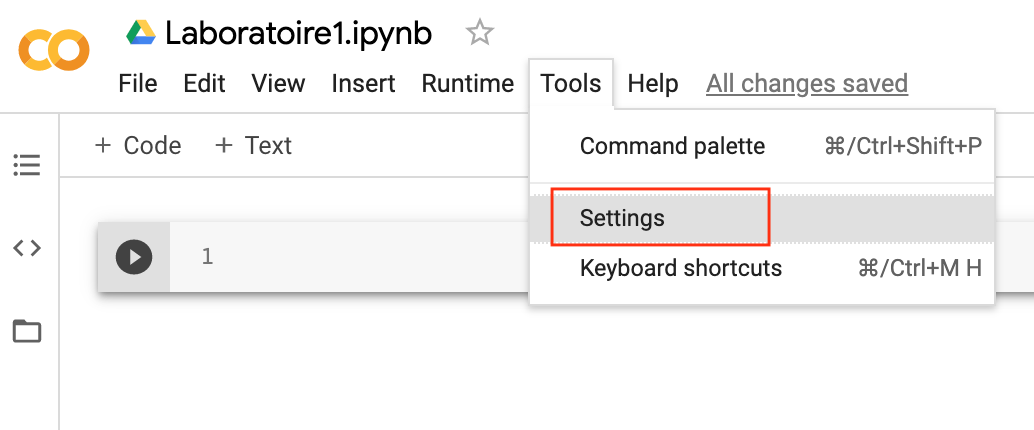
\includegraphics[width=0.75\linewidth]{figures/setting_menu}}
  \caption{Paramètres du notebook}
  \label{fig:setting}
\end{figure}

Dans le menu `Paramètres', vous êtes, par défaut, mis sur la page des paramètres du site (Figure \ref{fig:setting_site}). Dans cette page, il est possible de changer le thème afin qu'il devienne foncé et d'autoriser l'application \textit{Colaboratory} d'accéder aux répertoires privés sur un compte \textit{Github}. Cette dernière option peut être utile si vous prévoyez faire la gestion du laboratoire avec \textbf{Git}. Par défaut, \textit{Colaboratory} enregistre sur votre \textit{Google Drive} dans un fichier nommé `Colab Notebook'.

\begin{figure}[H]
  \centering
  \fbox{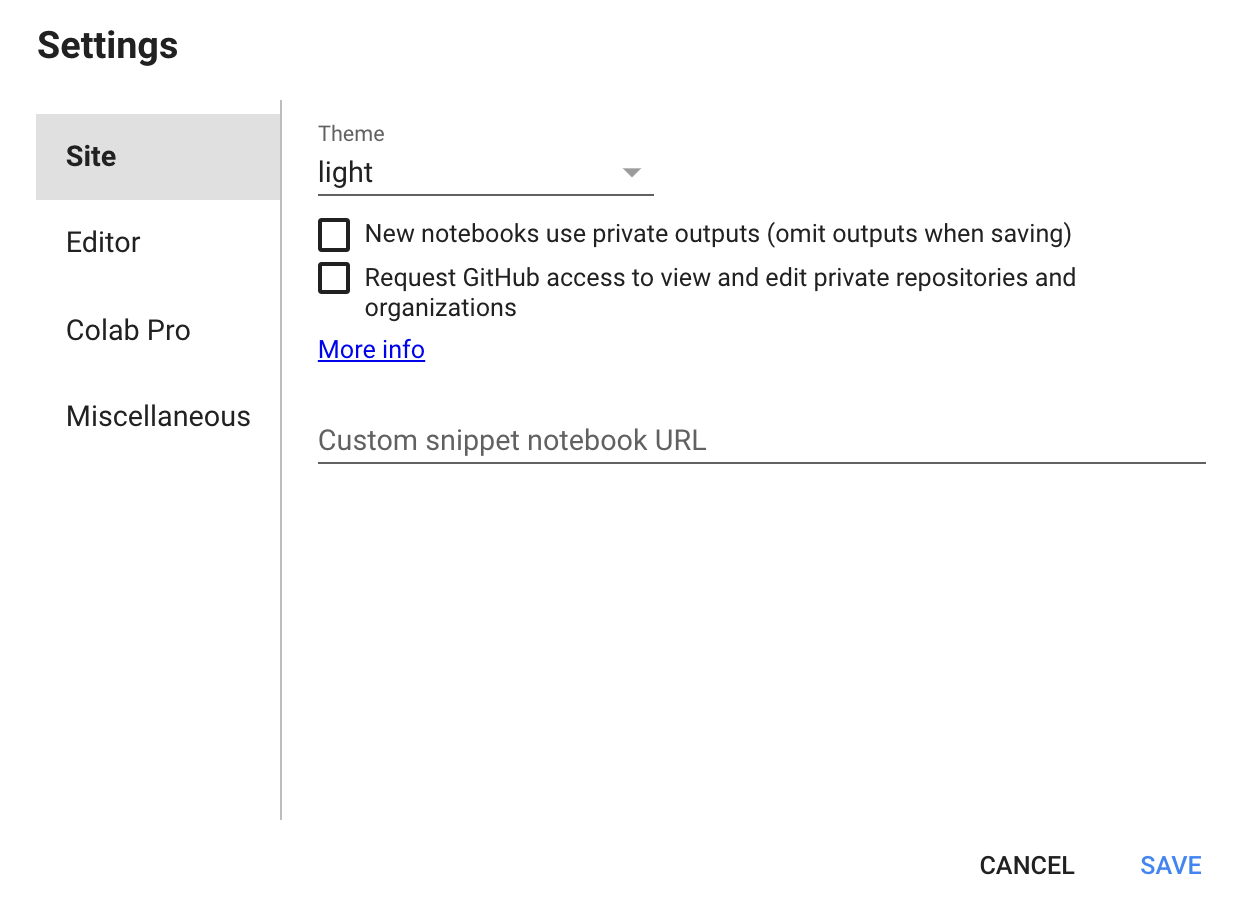
\includegraphics[width=0.75\linewidth]{figures/setting_site_menu}}
  \caption{Paramètres du site}
  \label{fig:setting_site}
\end{figure}

Dans l'onglet `Éditeur' (\textit{Editor}), assurez-vous que les options soient identiques à la figure \ref{fig:setting_editor}. Cela permet de faciliter la rédaction de code à l'intérieur du Notebook.

\begin{figure}[H]
  \centering
  \fbox{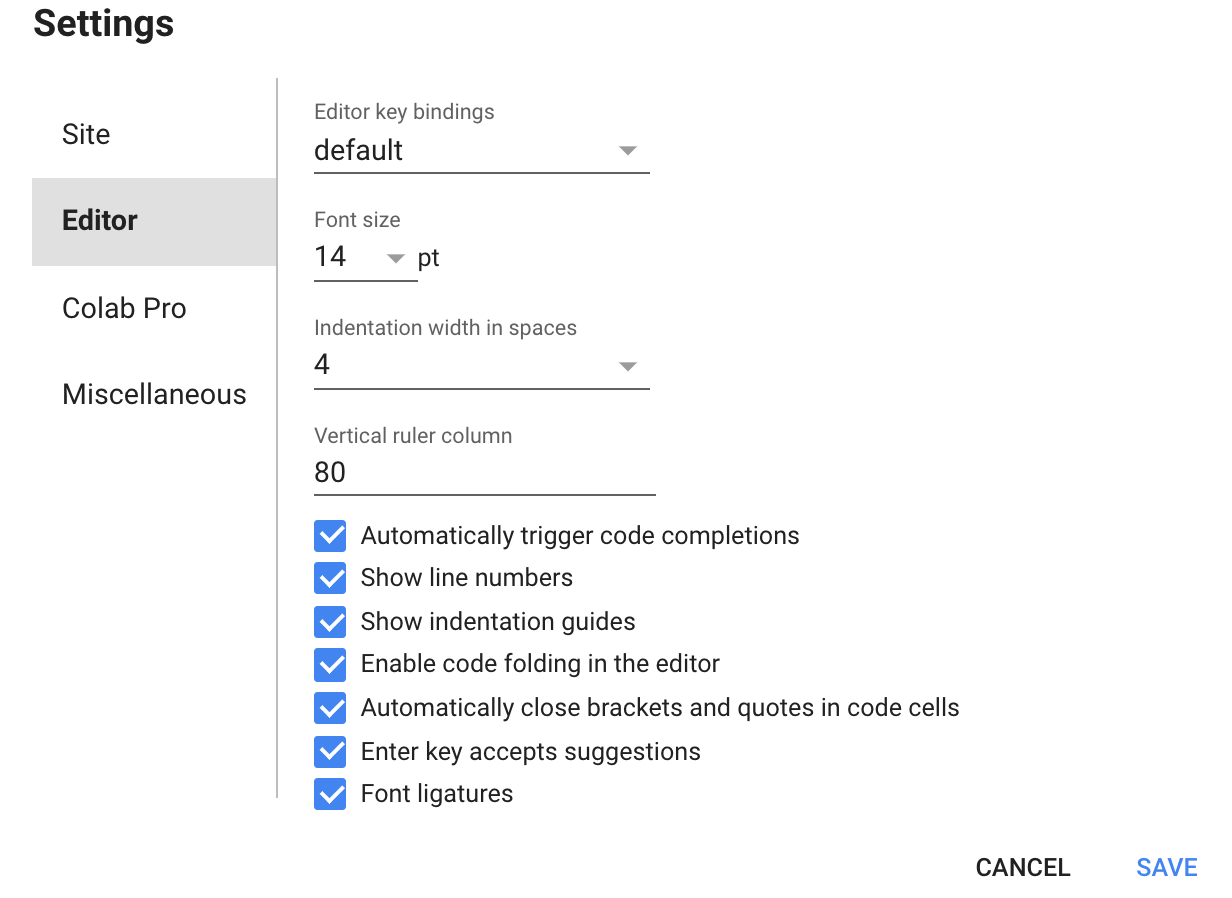
\includegraphics[width=0.75\linewidth]{figures/setting_editor_menu}}
  \caption{Paramètres de l'éditeur}
  \label{fig:setting_editor}
\end{figure}

\subsection{Ajouter une cellule de texte}

Pour ajouter une cellule dans votre notebook, vous pouvez déplacer votre curseur en haut ou en bas d'une cellule existante pour faire afficher l'option d'ajout (voir figure \ref{fig:add_cell}). Lorsqu'une cellule est sélectionnée, les boutons `+ Code' et `+ texte' ajoutent une cellule à la suite de la cellule sélectionnée. L'onglet `Insertion' (\textit{Insert}) offre des fonctionnalités similaires.
\medbreak
Pour déplacer une cellule, il suffit d'utiliser les icônes de flèches en haut à droite des cellules. Il est possible de déplacer plusieurs cellules consécutives en les sélectionnant.

\begin{figure}[H]
  \centering
  \fbox{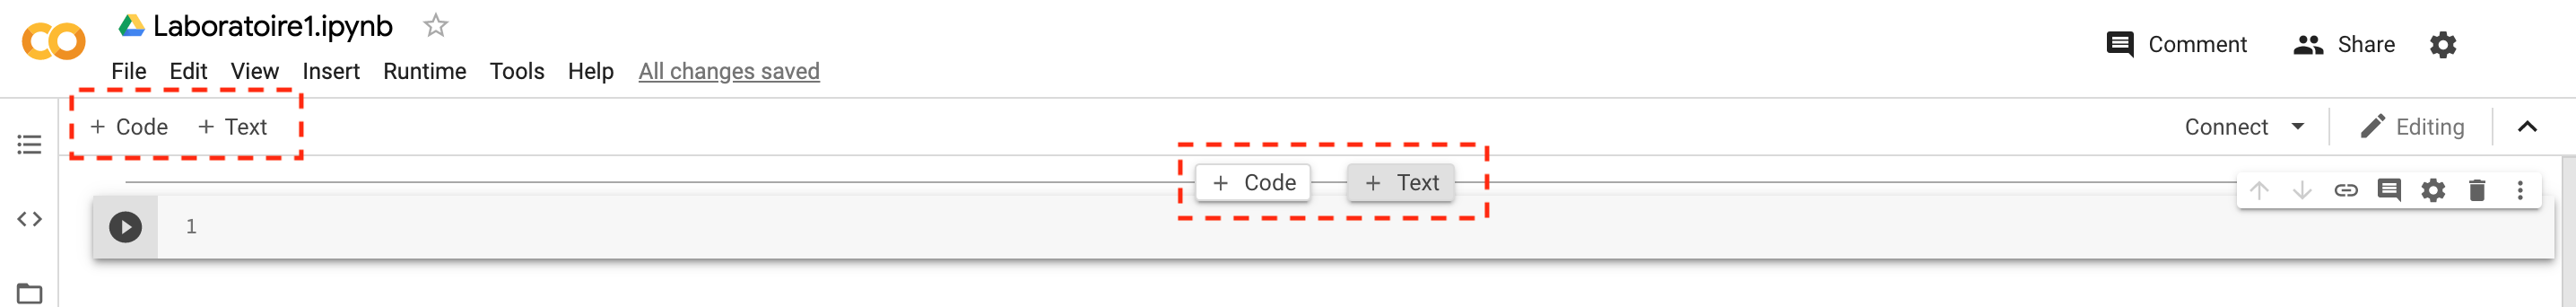
\includegraphics[width=0.75\linewidth]{figures/add_cell}}
  \caption{Ajouter une cellule}
  \label{fig:add_cell}
\end{figure}

Les cellules de texte sont utiles pour expliquer les résultats ou les théories d'une cellule de code. Les cellules de textes utilisent la nomenclature `Markdown' pour le texte et `LaTeX' pour les équations (exemple à la figure \ref{fig:add_text}).

\begin{figure}[H]
  \centering
  \fbox{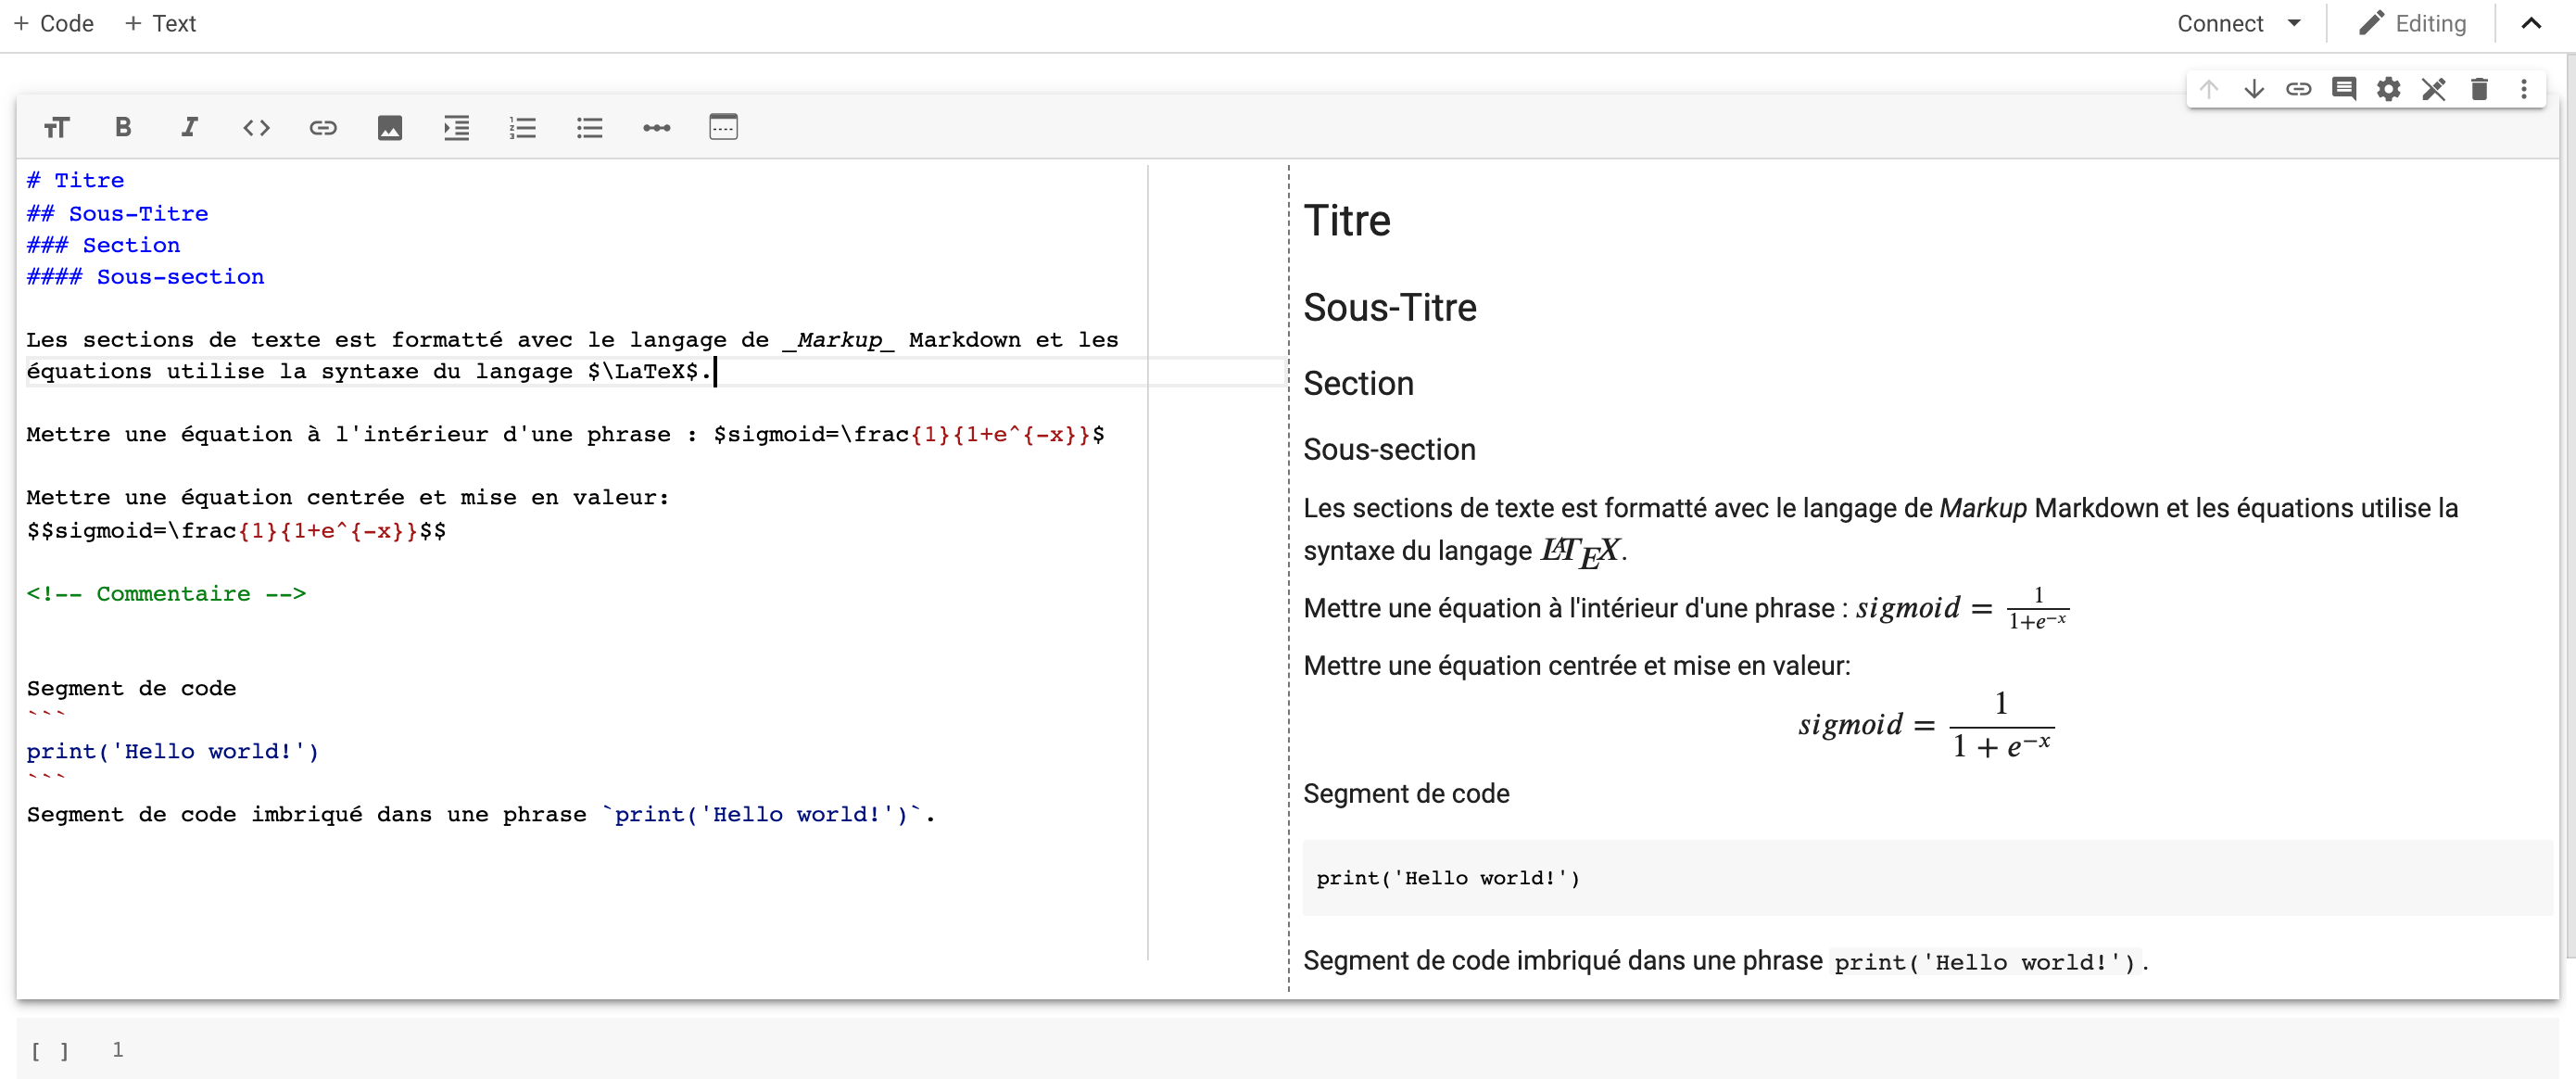
\includegraphics[width=0.75\linewidth]{figures/text_cell}}
  \caption{Ajouter une cellule de texte}
  \label{fig:add_text}
\end{figure}


\subsection{Ajouter une cellule de code}
Les cellules de code sont le coeur du notebook. Ces cellules utilisent \textbf{Python 3}.
\begin{figure}[H]
  \centering
  \fbox{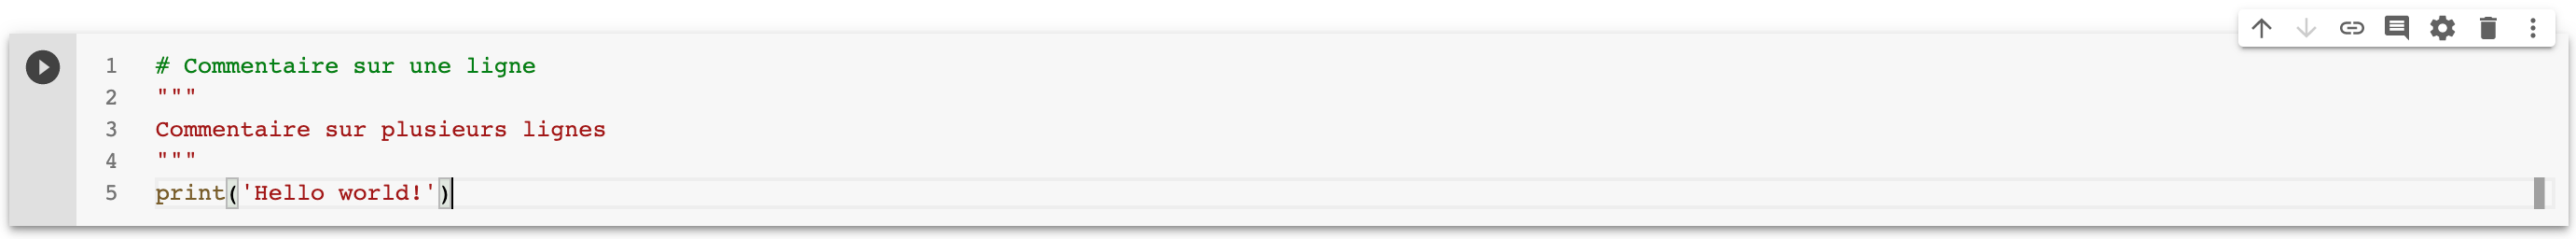
\includegraphics[width=0.75\linewidth]{figures/code_cell}}
  \caption{Ajouter une cellule de code}
  \label{fig:add_code}
\end{figure}


Pour exécuter individuellement une cellule de code, il suffit de cliquer sur l'icône en haut à gauche de la cellule (figure \ref{fig:code_run}). Davantage d'options d'exécution sont disponibles sous l'onglet `Exécution' (\textit{Runtime}) (figure \ref{fig:runtime_menu}). Le résultat de l'exécution est affiché sous la cellule. Les variables et fonctions d'une cellule sont accessibles après exécution pour les cellules de codes suivantes. En tout temps, il est possible d'arrêter le traitement d'une cellule de code en cliquant de nouveau sur l'icône d'exécution.

\begin{figure}[H]
  \centering
  \fbox{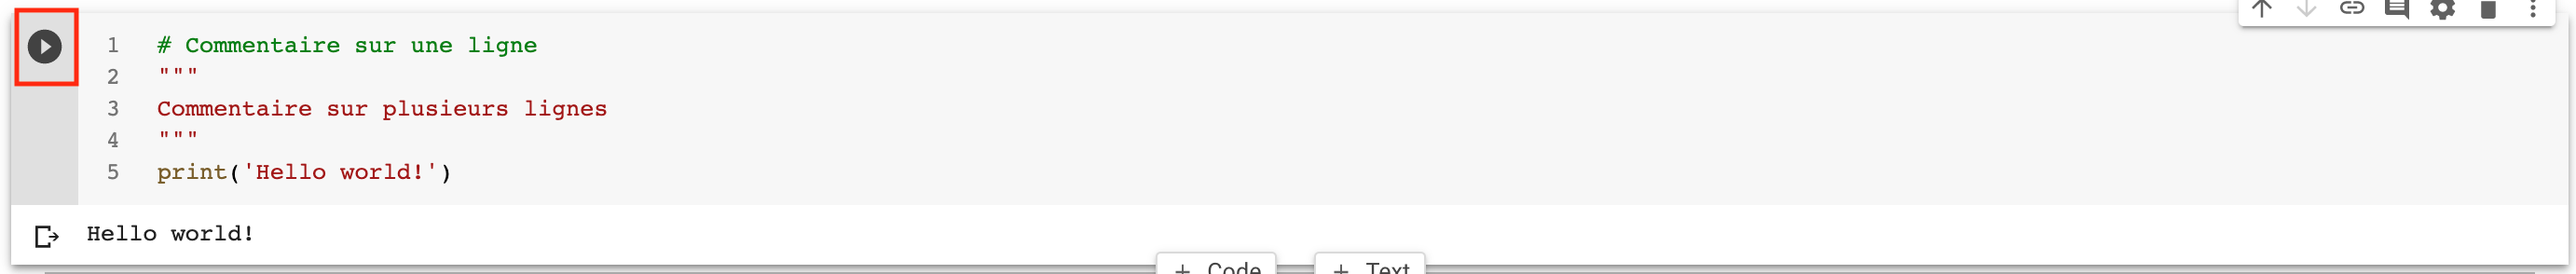
\includegraphics[width=0.75\linewidth]{figures/code_run}}
  \caption{Exécution d'une cellule de code}
  \label{fig:code_run}
\end{figure}

\begin{figure}[H]
  \centering
  \fbox{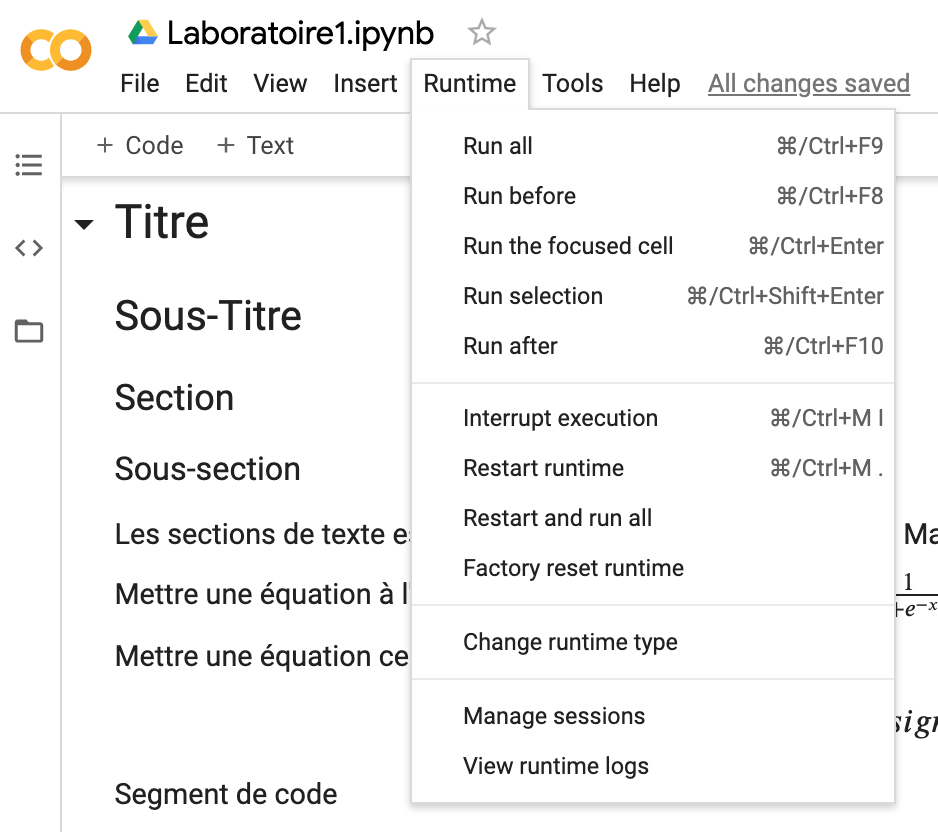
\includegraphics[scale=0.45]{figures/runtime_menu}}
  \caption{Menu d'exécution de cellules de code}
  \label{fig:runtime_menu}
\end{figure}

\textit{Le résultat à la dernière ligne d'une cellule de code est aussi affiché. Afin que le résultat de la dernière ligne ne soit pas affiché, ajouter `;' à la fin de la ligne.}
\medbreak
\textbf{Note : }\textit{lorsqu'un segment de code est demandé d'être retranscrit, ouvrez une nouvelle cellule de code afin de faciliter le déverminage (``debug'') en réduisant le temps d'exécution. Les segments de code sont conçus en sorte de respecter la norme PEP8, une description des fonctions est produite avec la structure du segment de codes de ce laboratoire \ref{code:nomenclature} et des commentaires sont ajoutés pour améliorer la compréhension des commandes. Après avoir retranscrit un segment de code, compilez la cellule de code.}
\medbreak
\begin{lstlisting}[language=Python, caption={Nomenclature de la description des fonctions}, label={code:nomenclature}]
def nom_de_la_fonction(argument1, argument2="valeur par defaut"):
    """
    NOM_DE_LA_FONCTION # en majuscule

    breve description de la fonction

    @Arguments :
      argument1 {type voulu pour l'argument1} : description de ce que doit etre l'argument1
      argument2 {type voulu pour l'argument2} : description de ce que doit etre l'argument2
        # (facultatif) explication du choix pour la valeur par defaut

    @Return :
      {type de l'objet retourne par la fonction} : description de l'objet retourne par la fonction
      # Si d'autres objets sont retournes, la meme syntaxe est utilisee pour chaque objet.

    (facultatif) Note : Information qui peut etre importante a connaitre pour l'utilisation de la fonction
    """
\end{lstlisting}
\medbreak

\subsection{Connecter à la machine virtuelle}

Afin de pouvoir compiler les cellules de code, il est nécessaire de se connecter à la machine virtuelle du notebook. Pour se faire, cliquez sur le bouton ``Connect'' en haut à droite du notebook tel que dans la figure \ref{fig:connect}.

\begin{figure}[H]
  \centering
  \fbox{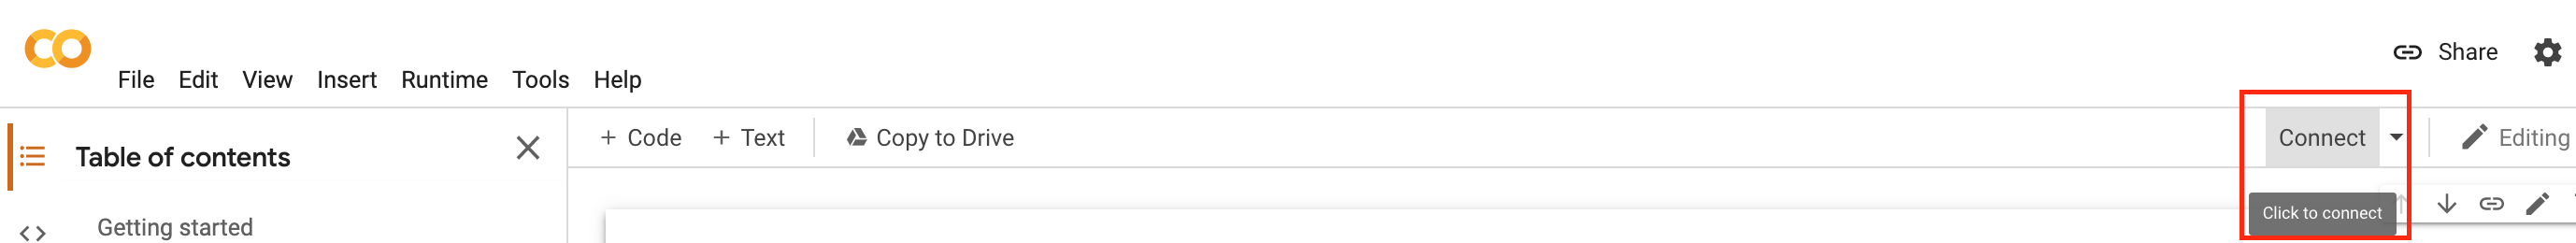
\includegraphics[width=0.75\linewidth]{figures/connect}}
  \caption{Connecter à la machine virtuelle du notebook}
  \label{fig:connect}
\end{figure}

\subsection{Importer les librairies}

Afin de produire les réseaux de neurones pour la classification des segments de la voix, il est primordial d'importer les librairies nécessaires. Dans la première cellule de code, copier les lignes du segment de codes \ref{code:import}.

\medbreak

\begin{lstlisting}[language=Python, caption={Importer les librairies}, label={code:import}]
import tensorflow as tf
from tensorflow.keras import layers
import numpy as np
import pandas as pd
import matplotlib.pyplot as plt
from scipy import stats
from sklearn.model_selection import KFold

# Pour l'affichage des figures sans plt.show()
%matplotlib inline
\end{lstlisting}


\subsection{Importer les bases de données}
Les bases de données utilisées dans le laboratoire sont disponibles sur le \textit{Moodle} de la classe. Après le téléchargement de ceux-ci, assurez-vous que le dossier est bien décompressé. Du côté gauche du notebook de Colaboratory (figure \ref{fig:onglet_gauche}), il y a trois onglets qui peuvent être utiles pour travailler avec le notebook. La première option est la table des matières du notebook. La table des matières est conçue automatiquement avec les titres dans les cellules de texte (figure \ref{fig:add_text}). La deuxième option est une cellule de recherche de segments de code compatible avec le notebook. La dernière option est un navigateur de dossiers pour les fichiers de la machine virtuelle où est placé le notebook.

\begin{figure}[H]
  \centering
  \fbox{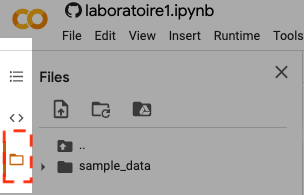
\includegraphics[scale=0.5]{figures/onglet_gauche}}
  \caption{Onglets du côté gauche du notebook}
  \label{fig:onglet_gauche}
\end{figure}

Sur l'onglet du navigateur de dossier, nous allons y déposer les fichiers ``training.csv'', ``test.csv'' et ``mystere.csv'' présents dans le fichier précédemment décompressé. Pour ce faire, il faut glisser-déposer (\textit{Drag and Drop}) directement dans la section de l'onglet fichier telle que dans la figure \ref{fig:dragndrop}. Il faut noter que Colaboratory n'accepte pas les dossiers pour le glisser-déposer. Alors, il faut sélectionner directement les trois fichiers à l'intérieur du fichier.

\begin{figure}[H]
  \centering
  \fbox{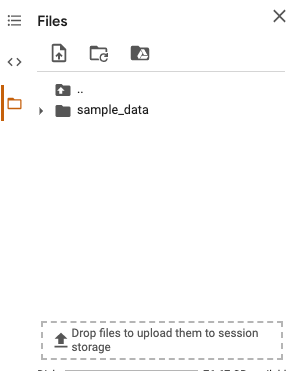
\includegraphics[scale=0.5]{figures/dragndrop}}
  \caption{Déposer les fichiers dans la barre de fichiers}
  \label{fig:dragndrop}
\end{figure}

Lorsque les fichiers y sont bien déposés, votre onglet ressemblera à celui de la figure \ref{fig:upload}.

\begin{figure}[H]
  \centering
  \fbox{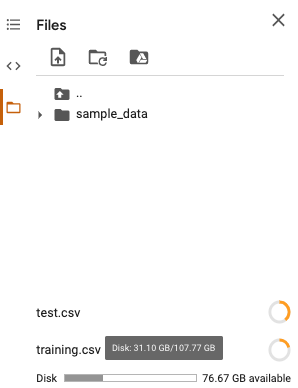
\includegraphics[scale=0.5]{figures/upload_files}}
  \caption{Importer les bases de données pour être accessible par le notebook}
  \label{fig:upload}
\end{figure}

Après que les fichiers sont importés, on peut vérifier qu'ils sont accessibles pour les prochaines étapes avec la commande suivante. Dans un notebook, lorsqu'une ligne de code commence avec un point d'exclamation (!), celle-ci réfère à une commande de terminal Linux. Dans le cas du segment de code \ref{code:lslah}, nous voulons afficher les fichiers sur le même niveau que le notebook.
\medbreak

\begin{lstlisting}[language=Python, caption={Voir les fichiers disponibles pour le notebook}, label={code:lslah}]
!ls -lah
\end{lstlisting}

\begin{figure}[H]
  \centering
  \fbox{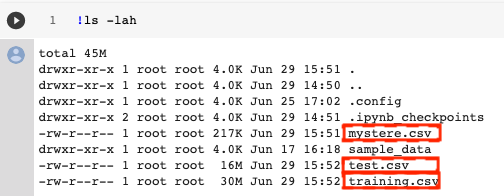
\includegraphics[scale=0.5]{figures/lslah}}
  \caption{Résultat de la commande ``ls -lah''}
  \label{fig:lslah}
\end{figure}

On voit bien, dans la figure \ref{fig:lslah}, les fichiers ``training.csv'', ``test.csv'' et ``mystere.csv''.

\subsection{Préparer les bases de données}
Pour que les bases de données soient accessibles au modèle, il faut utiliser la fonction de lecture de fichier ``.csv'' offert par la librairie \textit{Pandas} (Segment de codes \ref{code:read_ds}).
\smallbreak
\begin{lstlisting}[language=Python, caption={Lire les bases de données}, label={code:read_ds}]
# Transfert des datasets vers des variables (DataFrames)
train_ds = pd.read_csv("training.csv")
test_ds = pd.read_csv("test.csv")
\end{lstlisting}

La méthode `head' affiche les cinq premières valeurs d'une base de données. Tandis que la méthode `tail` affiche les cinq dernières. Pour obtenir les informations générales à propos d'une base de données, il suffit d'utiliser la méthode `info'.
\smallbreak

\begin{lstlisting}[language=Python, caption={Avoir de l'information de la base de données d'entraînement}, label={code:info_ds}]
print("__Train__")
print(train_ds.info())
print(train_ds.head())
print(train_ds.tail())
\end{lstlisting}

La figure \ref{fig:result_info_ds} est le résultat du segment de codes \ref{code:info_ds}.

\begin{figure}[H]
  \centering
  \fbox{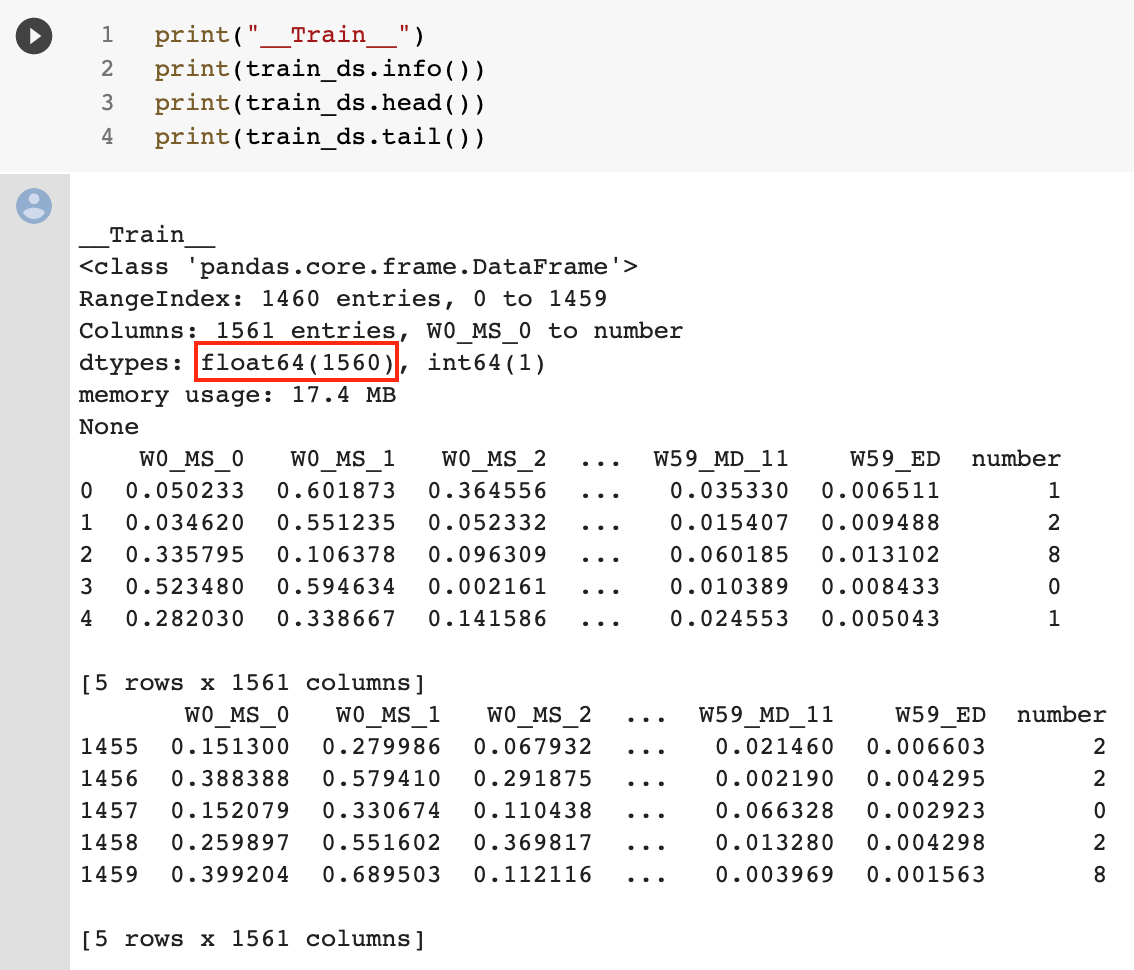
\includegraphics[width=0.75\linewidth]{figures/resultat_info_ds}}
  \caption{Résultat de la recherche d'information de la base de données d'entraînement}
  \label{fig:result_info_ds}
\end{figure}

Afin de concevoir la base de données de validation croisée avec la théorie du k-fold, nous allons concevoir une fonction (segment de codes \ref{code:create_ds}) qui sera, par la suite, utilisée dans la fonction d'entraînement (\textit{``training''}). Cette fonction retournera les bases de données d'entraînement, de validation croisée et de test formatées pour être directement utilisées dans la méthode ``fit'' du modèle de \textit{Tensorflow}. Le k-fold est une technique où la base de données d'entraînement est divisée en k parties. Avec cette segmentation, une des parties est utilisée pour des validations croisées et celles restantes seront utilisées pour l'entraînement du modèle.
\medbreak

\begin{lstlisting}[language=Python, caption={Création des bases de données pour l'entraînement}, label={code:create_ds}]
def create_sets(train_ds, test_ds, n_fold=5):
    """
    CREATE_SETS

    Transforme les bases de donnees afin d'etre compatible avec l'entrainement
    du modele avec la methode "fit"

    @Arguments :
        train_ds {pd.DataFrame} : Base de donnees d'entrainement
        test_ds {pd.DataFrame} : Base de donnees de test
        n_fold {int} : nombre de division pour le kfold

    @Return :
        {tensorflow.BatchDataset} : Base de donnees d'entrainement
        {tensorflow.BatchDataset} : Base de donnees de validation croisee
        {tensorflow.BatchDataset} : Base de donnees de test
    """
    # Melanger les valeurs de les bases de donnees
    train = train_ds.sample(frac=1).reset_index(drop=True)
    test  = test_ds.sample(frac=1).reset_index(drop=True)
    # Diviser les variables et les resultats
    train_output = train.pop("number")
    test_output = test.pop("number")

    # Extraire les indexes pour le kfold une seule fois
    for train_index, vc_index in KFold(n_fold).split(train) :
        # Creer la base de donnees d'entrainement
        X_train = (train.values)[train_index]
        y_train = (train_output.values)[train_index]

        # Creer la base de donnees de validation croisee
        X_vc = (train.values)[vc_index]
        y_vc = (train_output.values)[vc_index]

        # Creer la base de donnees de test
        X_test = test.values
        y_test = test_output.values
        break

    # Transformer les bases de donnees pour etre utilisees directement dans fit
    # Les donnees sont melangees une autre fois avant d'etre retournees
    train_set = tf.data.Dataset.from_tensor_slices((X_train, y_train))
    train_set = train_set.shuffle(len(X_train))
    train_set = train_set.batch(1)

    vc_set = tf.data.Dataset.from_tensor_slices((X_vc, y_vc))
    vc_set = vc_set.shuffle(len(X_vc))
    vc_set = vc_set.batch(1)

    test_set = tf.data.Dataset.from_tensor_slices((X_test, y_test))
    test_set = test_set.shuffle(len(X_test))
    test_set = test_set.batch(1)

    return train_set, vc_set, test_set
\end{lstlisting}

La fonction ``KFold'' utilisée à l'intérieur de ``create\_sets'' est conçue afin de produire k segmentations de bases de données. Dans notre cas, nous voulons faire qu'une seule segmentation, car le but n'est pas de faire l'évaluation du modèle, mais de montrer l'outil. Alors, la boucle ``for in'' est arrêtée après la première itération à l'aide du ``break''.

\subsection{Perceptron}
\subsubsection{Concevoir le modèle}
Dans ce laboratoire, on s'intéresse à concevoir des perceptrons multicouches (MLP). Ces réseaux de neurones sont séquentiels soit que la sortie d'une couche est l'entrée d'une seule autre couche. Dans ce laboratoire, la couche de sortie doit posséder 10 neurones pour respecter la quantité de classe dans les bases de données.
\medbreak
\textit{Dans ce laboratoire, on utilise la fonction de perte ``SparseCategoricalCrossentropy'' qui a la particularité de faire le calcul sur un vecteur où toutes les valeurs sont zéro sauf l'index de la valeur voulue qui est mis à un. Dans nos bases de données, il y a dix résultats possibles 0,1,2,3,4,5,6,7,8 et 9. Alors, les vecteurs de sortie doivent être de taille 1 par 10 (voir table \ref{tab:representation}). Pour cette raison, la dernière couche doit toujours posséder dix neurones.}

\begin{table}[H]
  \caption{Représentation vectorielle des nombres}
  \label{tab:representation}
  \centering
  \begin{tabular}{|c|c|}
    \hline
    Nombre & Représentation \\
    \hline
    0 & [1, 0, 0, 0, 0, 0, 0, 0, 0, 0] \\
    \hline
    1 & [0, 1, 0, 0, 0, 0, 0, 0, 0, 0] \\
    \hline
    2 & [0, 0, 1, 0, 0, 0, 0, 0, 0, 0] \\
    \hline
    3 & [0, 0, 0, 1, 0, 0, 0, 0, 0, 0] \\
    \hline
    4 & [0, 0, 0, 0, 1, 0, 0, 0, 0, 0] \\
    \hline
    5 & [0, 0, 0, 0, 0, 1, 0, 0, 0, 0] \\
    \hline
    6 & [0, 0, 0, 0, 0, 0, 1, 0, 0, 0] \\
    \hline
    7 & [0, 0, 0, 0, 0, 0, 0, 1, 0, 0] \\
    \hline
    8 & [0, 0, 0, 0, 0, 0, 0, 0, 1, 0] \\
    \hline
    9 & [0, 0, 0, 0, 0, 0, 0, 0, 0, 1] \\
    \hline
  \end{tabular}
\end{table}



\medbreak
Dans Tensorflow, les modèles sont construits à l'aide d'agrégation de couches offertes par la librairie Keras. Lorsque le modèle est conçu, il est nécessaire de le compiler (avec la méthode ``compile'') pour valider l'architecture pour l'entraînement. Afin de valider l'espace mémoire utiliser par les poids, il faut définir le datatype (dtype) de la couche. Dans notre cas, le \textit{dtype} des couches doivent être de ``float64'' pour ne pas nécessiter une conversion de type avec les valeurs en entrée (voir figure \ref{fig:zoom_result_info_ds})
\medbreak

\begin{figure}[H]
  \centering
  \fbox{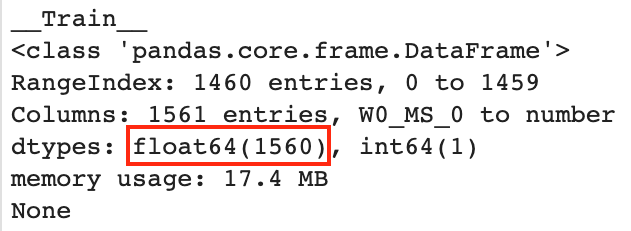
\includegraphics[width=0.75\linewidth]{figures/zoom_resultat_info_ds}}
  \caption{DataType de l'entrée}
  \label{fig:zoom_result_info_ds}
\end{figure}

Tel que vu en classe, la fonction d'optimisation utilisée est la descente de gradient. Dans la librairie Tensorflow, cet algorithme est référé par le sigle SGD (Descente de Gradient Stochastique). D'autres fonctions d'optimisation sont disponibles et sont majoritairement des variantes de SGD. La fonction de perte définie dans la compilation du modèle est le ``\textit{SparseCategoricalCrossentropy}''. Celle-ci est souvent utilisée pour la classification d'objet. La métrique observée dans notre cas est la précision du modèle. Soit, combien de fois le modèle obtient la bonne classe pour la donnée respective.
\medbreak
\begin{lstlisting}[language=Python, caption={Fonction pour l'entraînement du modèle}, label={code:create_perceptron}]
# Creer un modele sequentiel
perceptron = tf.keras.Sequential([
    layers.Dense(10, activation='sigmoid', dtype='float64')
])

# Compiler le modele pour l'entrainement
perceptron.compile(optimizer='SGD',
              loss= tf.keras.losses.SparseCategoricalCrossentropy(),
              metrics=['accuracy'])
\end{lstlisting}


\subsubsection{Concevoir une fonction personnalisée pour l'entraînement d'un modèle}
Afin d'identifier les rendements du modèle avec les trois bases de données, il est intéressant de concevoir une fonction personnalisée pour l'entraînement du modèle. Le but de cette fonction est qu'elle retourne les statistiques obtenues lors de l'entraînement. Python offre le dictionnaire (\textit{dict}) pour bien structurer les résultats. Les valeurs à l'intérieur d'un dictionnaire s'accèdent grâce aux clés de celui-ci (par exemple ``mon\_dict["ma\_cle"]''). Les clés du dictionnaire retourné par la fonction sont \textbf{train\_accuracy}, \textbf{train\_loss}, \textbf{vc\_accuracy}, \textbf{vc\_loss}, \textbf{test\_accuracy} et \textbf{test\_loss}.

\smallbreak
\begin{lstlisting}[language=Python, caption={Fonction pour l'entraînement du modèle}, label={code:training}]
def training(model, train_ds, test_ds, epochs=10, n_fold=5, verbose_train=1, verbose_vc=1, verbose_test=1):
    """
    TRAINING

    Fonction servant a entrainer un model tout en verifiant les capacites du modele
    sur les bases de donnees de validation croisee et de test

    @Arguments :
        model {tensorflow.python.keras.engine.sequential.Sequential} : Modele tensorflow a entrainer
        train_ds {pd.DataFrame} : Base de donnees d'entrainement
        test_ds {pd.DataFrame} : Base de donnnees de test
        epochs {int} : Nombre d'epoques a faire pour l'entrainement du model
        n_fold {int} : Nombre de fold pour le kfold
        verbose_train {int} : 1 pour afficher l'avancement de l'apprentissage, 0 aucun affichage
        verbose_vc {int} : 1 pour afficher l'avancement de l'evaluation, 0 aucun affichage
        verbose_test {int} : 1 pour afficher l'avancement de l'evaluation, 0 aucun affichage

    @Return:
        {dict} : 'train_accuracy' {list} : liste de la precision du modele sur la base de donnees d'entrainement
                  'train_loss' {list} : liste des resultat de la fonction de perte du modele sur la base de donnees d'entrainement
                  'vc_accuracy' {list} : liste de la precision du modele sur la base de donnees de validation croisee
                  'vc_loss' {list} : liste des resultats de la fonction de perte du modele sur la base de donnees de validation croisee
                  'test_accuracy' {list} : liste de la precision du modele sur la base de donnees de test
                  'test_loss' {list} : liste des resultats de la fonction de perte du modele sur la base de donnees de test
    """
    # Initialisation des listes recevants
    train_accuracy = []
    train_loss = []
    test_accuracy = []
    test_loss = []
    vc_accuracy = []
    vc_loss = []

    # Creer les bases de donnees pour l'entrainement
    train_set, vc_set, test_set = create_sets(train_ds, test_ds, n_fold)

    # Evaluer le modele avant l'entrainement
    result = model.evaluate(train_set, verbose=verbose_train)
    train_accuracy.append(result[1])
    train_loss.append(result[0])
    # ---
    result = model.evaluate(vc_set, verbose=verbose_vc)
    vc_accuracy.append(result[1])
    vc_loss.append(result[0])
    # ---
    result = model.evaluate(test_set, verbose=verbose_test)
    test_accuracy.append(result[1])
    test_loss.append(result[0])

    # Boucle d'entrainement
    for e in range(epochs):
        print('Epoch #{}'.format(e+1))
        # ---
        result = model.fit(train_set, epochs=1, verbose=verbose_train)
        train_accuracy.append(result.history['accuracy'][-1])
        train_loss.append(result.history['loss'][-1])
        # ---
        result = model.evaluate(vc_set, verbose=verbose_vc)
        vc_accuracy.append(result[1])
        vc_loss.append(result[0])
        # ---
        result = model.evaluate(test_set, verbose=verbose_test)
        test_accuracy.append(result[1])
        test_loss.append(result[0])

    return {'train_accuracy':train_accuracy,
            'train_loss':train_loss,
            'vc_accuracy':vc_accuracy,
            'vc_loss':vc_loss,
            'test_accuracy':test_accuracy,
            'test_loss':test_loss}
\end{lstlisting}

\subsubsection{Concevoir une fonction personnalisée pour afficher les statistiques de l'entraînement}
Après l'entraînement d'un modèle, nous voulons savoir comment a été l'apprentissage du modèle. Pour ce faire, il est primordial de produire une figure affichant les statistiques produites par l'entraînement. Comme nous avons créé une fonction précédemment pour l'entraînement de modèle, nous pouvons utiliser les résultats de celui-ci. La fonction ``training'' retourne un dictionnaire avec un formatage précis qui sera facile à manipuler. Cette fonction réduira la manipulation pour les prochaines étapes.
\medbreak
\begin{lstlisting}[language=Python, caption={Fonction pour l'affichage des statistiques de l'entraînement}, label={code:figure}]
def figure(training_dict, suptitle, figsize=(12,6)):
    """
    FIGURE

    Produit une figure avec les statistiques de la fonction 'training'

    @Arguments :
        training_dict {dict(list)} : Dictionnaire retournee par la fonction training
        figsize {Tuple} : Dimension de la figure
    """
    # Demarre une figure avec la taille (en pouce) donner en arguments
    plt.figure(figsize=figsize,facecolor='w')

    # Titre global de la figure
    plt.suptitle(suptitle)

    # Premiere sous-figure -> Precision du modele durant l'entrainement
    plt.subplot(121)
    plt.title('Precision du modele')
    plt.xlabel('Nombre d\'epoques')
    plt.ylabel('Precision de la classification')
    # Produit une courbe pour chaque base de donnees
    plt.plot(training_dict['train_accuracy'], 'r', label='training')
    plt.plot(training_dict['vc_accuracy'], 'b--', label='vc')
    plt.plot(training_dict['test_accuracy'], 'y', label='test')
    # Limite de la precision pour rendre les valeurs entre 0% et 100% visibles
    plt.ylim(0,1.01)
    # Produire un grille en arriere-plan
    plt.grid(b=True, which='major', color='#666666', linestyle='-')
    plt.minorticks_on()
    plt.grid(b=True, which='minor', color='#999999', linestyle='-', alpha=0.2)
    plt.legend() # Afficher les labels des courbes

    # Deuxieme sous-figure -> Resultat de la fonction de perte durant l'entrainement
    plt.subplot(122)
    plt.title('Perte du modele')
    plt.xlabel('Nombre d\'epoques')
    plt.ylabel('Resultat de la fonction de perte')
    # Produire une courbe pour chaque base de donnees
    plt.plot(training_dict['train_loss'],'r', label='training')
    plt.plot(training_dict['vc_loss'],'b--', label='vc')
    plt.plot(training_dict['test_loss'],'y', label='test');
    # S'assurer que la valeur minimum de l'ordonnee soit 0
    plt.ylim(0);
    # Produire un grille en arriere-plan
    plt.grid(b=True, which='major', color='#666666', linestyle='-')
    plt.minorticks_on()
    plt.grid(b=True, which='minor', color='#999999', linestyle='-', alpha=0.2)
    plt.legend()
    return
\end{lstlisting}
\textit{La fonction ``plt.subplot()'' a comme argument un chiffre qui correspond à la disposition des sous-figures. La centaine indique combien de rangées de sous-figures seront dans la figure. La dizaine est pour le nombre de colonnes de sous-figures. Dans notre cas, nous  aurons deux figures mises côte à côte telle que dans la figure \ref{fig:ex_figure}. L'unité correspond à quelle est la sous-figure qui nous voulons formater.}

\begin{figure}[H]
  \centering
  \fbox{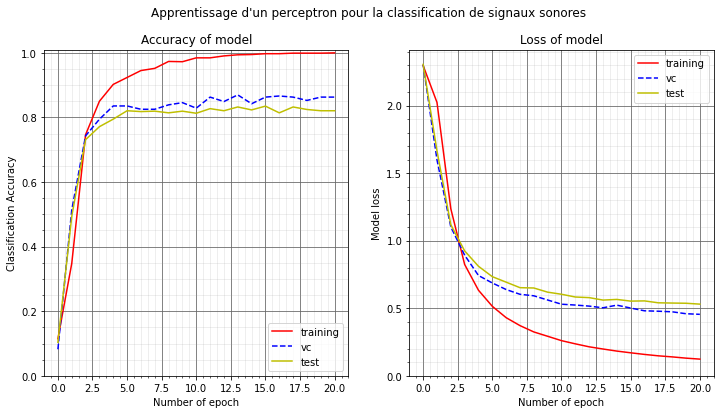
\includegraphics[width=0.75\linewidth]{figures/example_figure}}
  \caption{Figure produite par la fonction ``figure''}
  \label{fig:ex_figure}
\end{figure}

\subsubsection{Entraîner le modèle}
Avec la fonction ``training'' conçue précédemment, il est facile de faire l'entraînement du perceptron. Il suffit de mettre la variable contenant le perceptron, les deux bases de données (\textit{train\_ds et test\_ds}) et le nombre d'époques voulu pour l'entraînement dans la fonction comme ci-dessous.
\smallbreak
\begin{lstlisting}[language=Python, caption={Entraînement du perceptron}, label={code:train_perceptron}]
result = training(perceptron, train_ds, test_ds, epochs=25)
\end{lstlisting}
\medbreak
Il est possible de réduire le nombre d'affichages dans la console à l'aide des arguments de verbose de la fonction ``training''.

\subsubsection{Afficher les statistiques du modèle}
La fonction ``figure'' linéarise l'affichage graphique des résultats obtenus durant l'entraînement.
\smallbreak
\begin{lstlisting}[language=Python, caption={Affichage des résultats de l'entraînement}, label={code:display_perceptron}]
figure(result, "Apprentissage d'un perceptron pour la classification des signaux sonores")
\end{lstlisting}

\begin{figure}[H]
  \centering
  \fbox{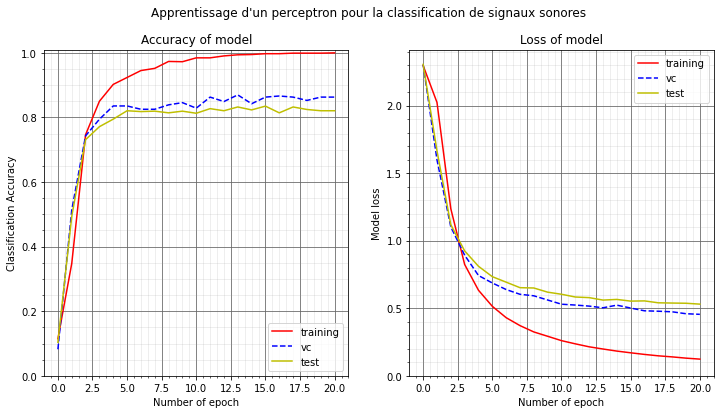
\includegraphics[width=0.75\linewidth]{figures/example_figure}}
  \caption{Affichage des graphiques avec les résultats de l'entraînement du perceptron}
  \label{fig:stats_figure}
\end{figure}

\subsubsection{Enregistrer le modèle}
Afin de ne pas perdre ce perceptron, il est nécessaire de l'enregistrer. Tensorflow possède sa propre structure pour sauvegarder un modèle. Pour ce faire, il faut faire appel à la méthode ``save''. Cette méthode nécessite le nom désiré pour le fichier de sauvegarde. Je recommande de mettre tous les fichiers de  sauvegarde dans un seul dossier. Dans le segment de code \ref{code:save_perceptron}, la sauvegarde est nommée ``perceptron'' et est mise à l'intérieur du dossier ``modeles'.
\medbreak
\begin{lstlisting}[language=Python, caption={Enregistrer le Perceptron}, label={code:save_perceptron}]
perceptron.save('modeles/perceptron')
\end{lstlisting}

\subsection{MLP à deux couches}
% TODO : Pourquoi il est intéressant d'ajouter une couche supplémentaire? - Question rapport
Après la création d'un perceptron, il est intéressant de voir qu'est-ce que peut apporter une couche supplémentaire à la classification des données.
\subsubsection{Concevoir le modèle}
Avec les connaissances développées pour la création du perceptron, faites la conception d'un perceptron multicouche (MLP) de deux couches. Après l'entraînement, il est possible de vérifier la structure du modèle avec la méthode ``\textbf{summary}''.
\medbreak

\begin{lstlisting}[language=Python, caption={Conception d'un perceptron multicouches}, label={code:add_layer}]
mlp2c = tf.keras.Sequential([
    layers.Dense(512, activation='sigmoid', dtype='float64'),
    layers.Dense(10, activation='sigmoid', dtype='float64')
])

# Compiler le modele pour l'entrainement
mlp2c.compile(optimizer='SGD',
              loss= tf.keras.losses.SparseCategoricalCrossentropy(),
              metrics=['accuracy'])
\end{lstlisting}

Le segment de codes \ref{code:new_tech} est une technique utilisée pour produire des réseaux neurones avec un architecture plus flexible. Cette technique sera plus pertinente dans les prochains laboratoires.

\begin{lstlisting}[language=Python, caption={Conception d'un perceptron multicouches (technique supplémentaire)}, label={code:new_tech}]
# Creer une couche d'entree
# La dimension des Tensors utilises est de (None, 1, 1560)
model_input = layers.Input(shape=(None, 1, train_ds.shape[1]-1))

# Creer les couches du reseau de neurones
x = layers.Dense(512, activation='sigmoid',dtype='float64')(model_input)
model = layers.Dense(10, activation='sigmoid', dtype='float64')(x)

# Valider le modele
model = tf.keras.Model(model_input, model)

# Compiler le modele pour l'entrainement
model.compile(optimizer='SGD',
              loss= tf.keras.losses.SparseCategoricalCrossentropy(),
              metrics=['accuracy'])
\end{lstlisting}


\medbreak
La valeur de neurones dans la première couches n'est pas forcée telle que celle de la dernière couche. Alors, il est possible de la modifier afin de voir l'effet qu'ont les différentes quantité de neurones.
\medbreak

\begin{figure}[H]
  \centering
  \fbox{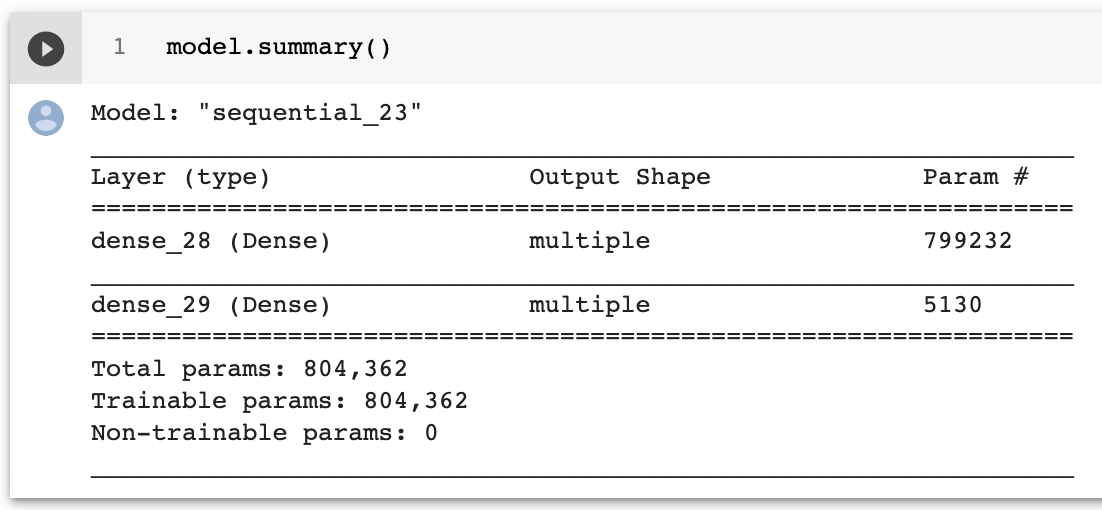
\includegraphics[width=0.75\linewidth]{figures/summary}}
  \caption{Exemple de l'utilisation de la méthode ``summary'' sur un modèle de deux couches denses}
  \label{fig:summary}
\end{figure}

\subsubsection{Entraîner le modèle}
Faites l'entraînement du MLP à deux couches à l'aide de la fonction ``training''.
\medbreak
\textit{Si vous obtenez des erreurs lors de l'entraînement, assurez-vous qu'il ait bien dix neurones pour la couche en sortie.}
\subsubsection{Afficher les statistiques du modèle}
Affichez les résultats obtenus durant l'entraînement du MLP.
\subsubsection{Enregistrer le modèle}
Sauvegardez le modèle entraîné sous le même dossier avec le nom ``mlp2c'' pour MLP à deux couches.

\subsection{MLP à deux couches et une couche d'abandon}
Une problématique avec l'entraînement est le surentraînement soit lorsque le modèle se spécialise davantage sur les données que sur le concept. Une des solutions pour palier au surentraînement est l'ajout d'une couche d'abandon ou selon le terme original ``Dropout'' (\cite{Dropout-article}).
\subsubsection{Concevoir le modèle}
Pour le laboratoire, nous allons mettre la couche d'abandon entre les deux couches totalement connectées (``Dense''). De cette manière, la dernière couche devra prendre en compte des données manquantes de la couche précédente pour concevoir un choix. Ajoutez la couche suivante entre les deux couches ``Dense''.
\medbreak

\begin{lstlisting}[language=Python, caption={Appel de la couche Dropout}, label={code:dropout_layer}]
layers.Dropout(0.2, dtype='float64')
\end{lstlisting}
\medbreak

Le premier argument pour l'initialisation de la couche Dropout est le pourcentage (entre 0 et 1) d'abandon de la couche précédente. L'abandon des neurones sera fait aléatoirement.

\subsubsection{Entraîner le modèle}
Faites l'entraînement du MLP à deux couches avec abandon à l'aide de la fonction ``training''.
\medbreak
\textit{Si vous obtenez des erreurs lors de l'entraînement, assurez-vous qu'il ait bien dix neurones pour la couche en sortie et que toutes les couches sont du même dtype.}
\subsubsection{Afficher les statistiques du modèle}
Affichez les résultats obtenus durant l'entraînement du MLP avec abandon.
\subsubsection{Enregistrer le modèle}
Sauvegardez le modèle entraîné sous le même dossier avec le nom ``mlp2cd''.

\subsection{MLP à trois couches}
Après l'entraînement fait avec les perceptrons multicouches à deux couches, il est intéressant de voir qu'est-ce que peut apporter une autre couche supplémentaire à la classification des données.
\subsubsection{Concevoir le modèle}
Avec les connaissances développées précédemment, faites la conception d'un perceptron multicouches (MLP) de trois couches sans couches d'abandon. Après l'entraînement, il est possible de vérifier la structure du modèle avec la méthode ``\textbf{summary}''.

\subsubsection{Entraîner le modèle}
Faites l'entraînement du MLP à trois couches à l'aide de la fonction ``training''.
\medbreak
Si vous obtenez des erreurs lors de l'entraînement, assurez-vous qu'il ait bien dix neurones pour la couche en sortie.
\medbreak

\textit{Lorsque la profondeur d'un modèle augmente, on peut apercevoir l'effet de la disparition du gradient. Celle-ci est causé par la fonction d'activation utilisée dans les couches du modèle. La disparition de gradient réfère au gradient qui tend vers zéro lorsque ses arguments tendent vers l'infini (positif ou négatif) (voir figure \ref{fig:dsigmoid}). Une fonction pouvant créer une disparition des gradients est la fonction sigmoïde. Une technique pour corriger la situation est d'utiliser la fonction d'activation ``relu'' au lieu de ``sigmoïde'' et d'ajouter une couche ``Softmax'' au modèle.}

\begin{figure}[H]
\centering
\begin{minipage}{.5\textwidth}
  \centering
  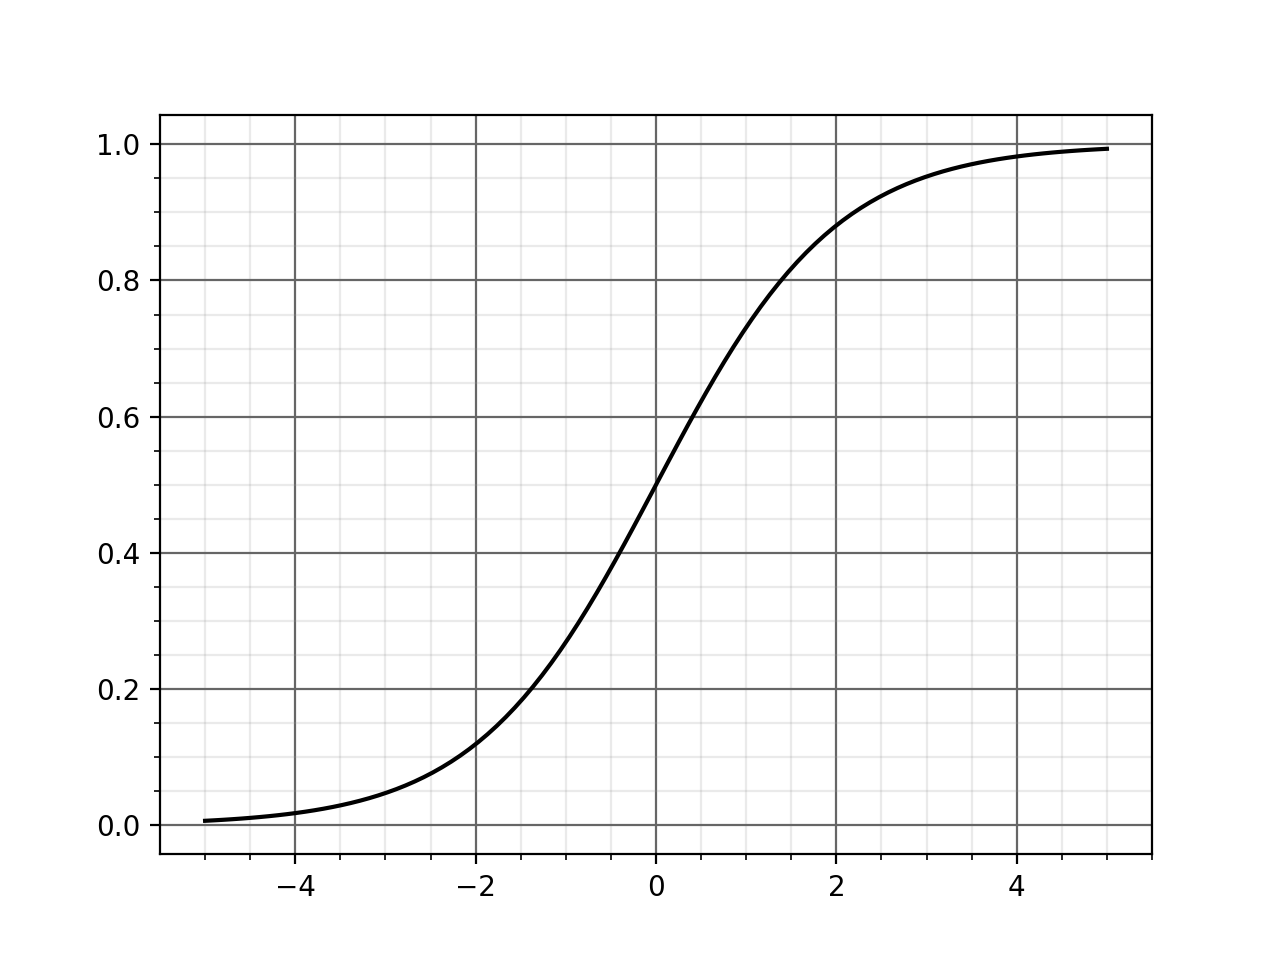
\includegraphics[width=1\linewidth]{Figures/sigmoid.png}
  \captionof{figure}{Fonction d'activation Sigmoïde}
  \label{fig:sigmoid}
\end{minipage}%
\begin{minipage}{.5\textwidth}
  \centering
  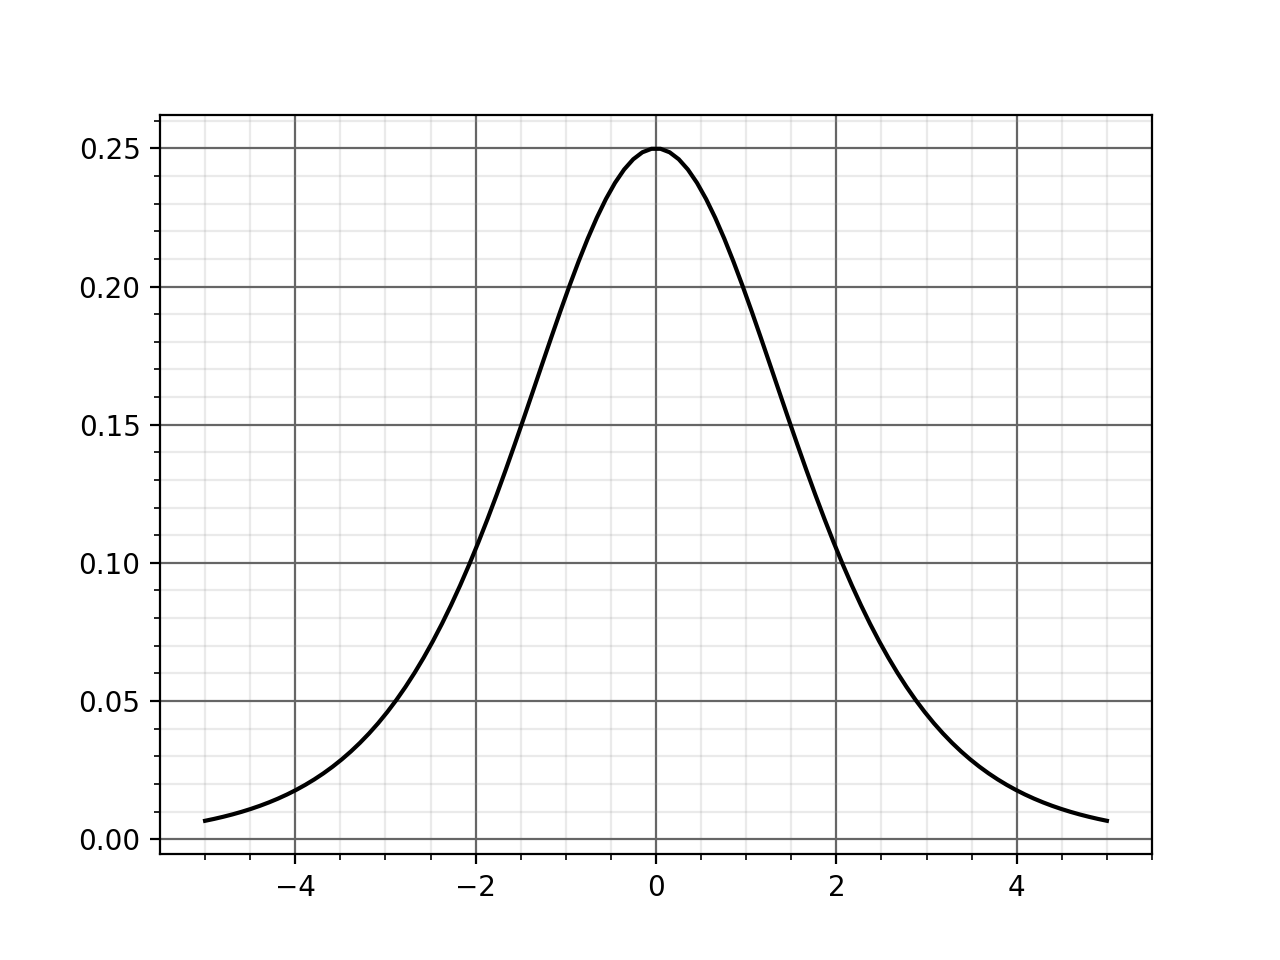
\includegraphics[width=1\linewidth]{Figures/sigmoid_derivate.png}
  \captionof{figure}{Dérivée de la fonction d'activation Sigmoïde}
  \label{fig:dsigmoid}
\end{minipage}
\end{figure}

Afin que votre MLP à trois couches puisse classifier les signaux sonores, changez le modèle pour celui du segment de code \ref{code:vanish_grad} et faites l'entraînement de celui-ci.
\medbreak

\begin{lstlisting}[language=Python, caption={Correction de la disparition du gradient}, label={code:vanish_grad}]
mlp3c = tf.keras.Sequential([
    layers.Dense(512, activation='relu', dtype='float64'),
    layers.Dense(128, activation='relu', dtype='float64'),
    layers.Dense(10, activation='relu', dtype='float64'),
    layers.Softmax(dtype='float64')
])
\end{lstlisting}

\subsubsection{Afficher les statistiques du modèle}
Affichez les résultats obtenus durant l'entraînement du MLP à l'aide de la fonction ``figure''.
\subsubsection{Enregistrer le modèle}
Sauvegardez le modèle entraîné sous le même dossier avec le nom ``mlp3c''.

\subsection{Déterminer la classe des segments audios mystères}
% Les fichiers audios mystères sont pour les valeurs 2, 0, 8, 2, 1, 0, 8, 2, 5 et 4.
Une troisième base de données a été offerte pour simuler la mise en production d'un modèle. Pour ce faire, cette base de données ne possède pas la colonne ``number'' référant à la signification du signal sonore. Afin de savoir qu'elle est le résultat correspondant à ces données, il serait intéressant de voir quels sont les résultats prédits par les modèles entraînés durant le laboratoire.

\begin{lstlisting}[language=Python, caption={Chargement de la base de données mystères}, label={code:load_data}]
_mystere_ds = pd.read_csv("mystere.csv")
print(_mystere_ds.info())
mystere_ds = tf.data.Dataset.from_tensor_slices(_mystere_ds.values)
mystere_set = mystere_ds.batch(1)
\end{lstlisting}

\begin{lstlisting}[language=Python, caption={Chargement du perceptron}, label={code:load_model}]
# Chargement du perceptron entraine precedement
model =  tf.keras.models.load_model('modeles/perceptron')
# Obtenir seulement l'index de la valeur la plus grande de la reponse du modele
np.argmax(model.predict(mystere_set), axis=1)
\end{lstlisting}

Afin de voir les résultats obtenus pour tous les modèles du laboratoire, nous pouvons utiliser une boucle ``for in''.

\begin{lstlisting}[language=Python, caption={Prédire le résultat des données avec tous les modèles}, label={code:predict}]
# Concevoir une liste vide prete a recevoir les resultats
result = []
# Voir la prediction de chaque modele
for model_dir in ['modeles/perceptron','modeles/mlp2c','modeles/mlp2cd','modeles/mlp3c']:
    model = tf.keras.models.load_model(model_dir)
    prediction = model.predict(mystere_set)
    # Retourne l'index ayant la plus grande valeur
    result.append(np.argmax(prediction, axis=1))

# Transferer la liste en array de numpy
result = np.array(result)

# Afficher les resultats
print("Resultat de tous les modeles")
print(result)
print("Resultat commun entre les modeles")
print((stats.mode(result, axis=0))[0])
\end{lstlisting}

Une fonctionnalité a noté est d'ajouté une couche ``Softmax'' à la suite d'un modèle avec la méthode ``add''. Le segment de codes \ref{code:add} fait que les valeurs en sortie du réseau de neurones est la probabilité que la sortie soit une classe donnée comparativement à une valeur arbitraire tel que donnée lors de l'entraînement.
\medbreak
\begin{lstlisting}[language=Python, caption={Utilisation de la méthode ``add''}, label={code:add}]
model.add(layers.Softmax(dtype='float64'))
# Recompiler le modele afin qu'il puissent faire la prediction
model.compile(optimizer='SGD',
              loss= tf.keras.losses.SparseCategoricalCrossentropy(),
              metrics=['accuracy'])
\end{lstlisting}

\section{À mettre dans le rapport} % Document à remettre
Avec le rapport, il faut remettre le notebook (`.ipynb') et le dossier ``modeles''
\medbreak

Pour télécharger le fichier du notebook, cliquez l'option ``Télécharger .ipynb'' (\textit{``Download .ipynb''}) sous l'onglet fichier.

\begin{figure}[H]
  \centering
  \fbox{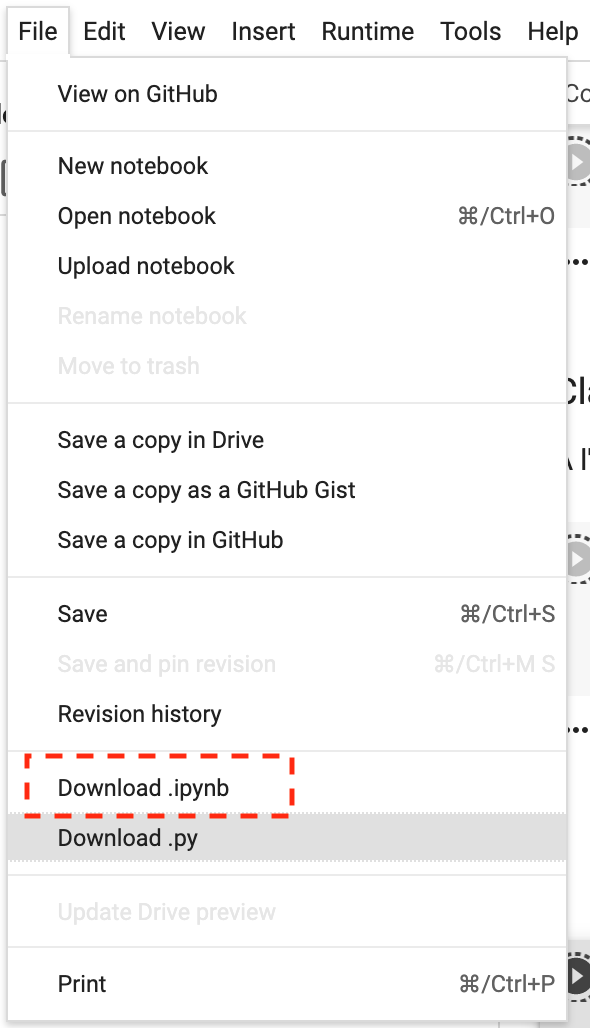
\includegraphics[height=0.75\linewidth]{figures/downloadipynb}}
  \caption{Télécharger le notebook}
  \label{fig:downloadipynb}
\end{figure}
\medbreak
Afin de télécharger le dossier ``modeles'', il faut le compresser auparavant. Pour se faire, ouvrer une nouvelle cellule de code et insérer la commande ci-dessous.

\begin{lstlisting}[language=Python, caption={Compresser un fichier sur une session}, label={code:zip}]
!zip -r modeles.zip ./modeles
\end{lstlisting}
\smallbreak
\textit{Faites attention au point d'exclamation [!] au début de la commande}

\medbreak
Par la suite, il est possible de télécharger en se dirigeant sur l'icône de fichier dans la barre de gauche du notebook tel que représenté dans la figure \ref{fig:downloadzip}.
\begin{figure}[H]
  \centering
  \fbox{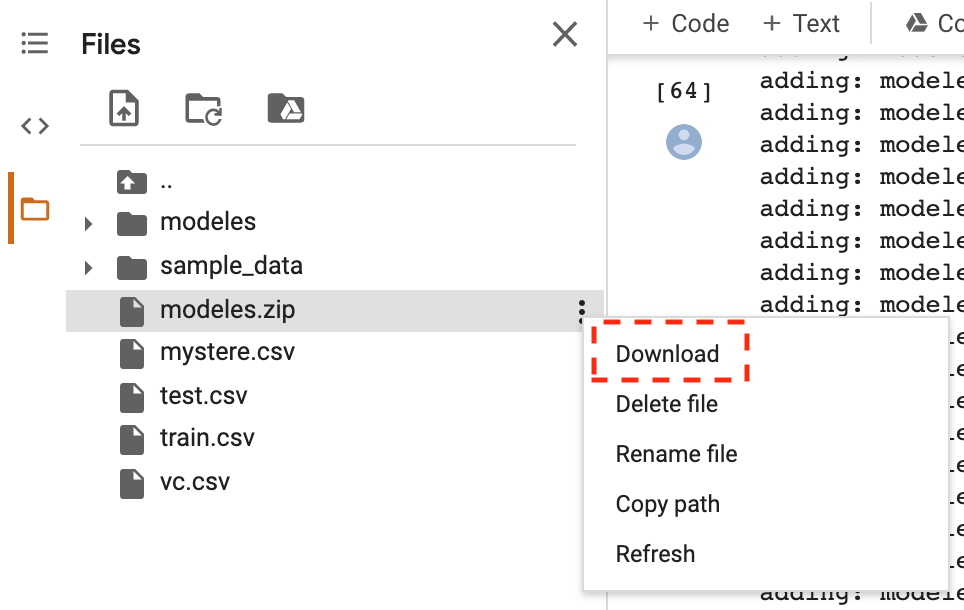
\includegraphics[width=0.75\linewidth]{figures/downloadzip}}
  \caption{Télécharger le dossier compressé}
  \label{fig:downloadzip}
\end{figure}

\begin{table}[H]
  \caption{Contenu du rapport}
  \label{tab:remettre}
  \centering
  \begin{tabular}{|l|l|l|c|}
    \hline
    Section & Taille minimum & Pondération \\
    \hline
    Introduction & 3 lignes & 5\%\\
    Théorie & 5 lignes & 20\%\\
    Résultats & 5 lignes & 40\%\\
    Conclusion & 5 lignes & 35\%\\
    \hline
  \end{tabular}
\end{table}

\subsection{Description des sections}
\subsubsection{Introduction}
Dans l'introduction, il faut décrire le but du laboratoire et de résumer la procédure du laboratoire.

\subsubsection{Théorie}
Dans la section théorique, il est nécessaire d'expliquer les théories et les concepts qui sont mis de l'avant par le laboratoire.

\subsection{Résultats}
La section des résultats doit inclure les graphiques, les tableaux obtenus durant le laboratoire. Il est nécessaire d'inclure une figure décrivant l'entrainement pour chaque modèle. De plus, il est nécessaire d'expliquer le résultat observé à l'intérieur de la figure.

\subsubsection{Conclusion}
Finalement, la conclusion doit contenir un simple retour sur le but, une évaluation des résultats et une ouverture sur l'amélioration du laboratoire.


\bibliography{references}

\end{document}
